\chapter{Deep Neural Network Functions}
\input{3FEM/FEspaces}
\input{6DL/FEM2DNN}
\input{6DL/WhyDeep}
\input{6DL/DNN}
\input{6DL/DefineDNN} 

In this chapter, we will discuss a number of activation functions.  We
say an activation function $\alpha$ 
satisfies the basic activated-approximation-property (AAP) if for any $g\in C^1[-1,1]$, we have
\begin{equation}
\label{AAP}
\min_{a_i,b_i,c,w_i\in\mathbb R^1}\max_{t\in[-1,1]}\bigg|g(t)-\sum_{i=1}^k(a_i\alpha(w_it+b_i)-c\bigg|
\le \frac{C}{k}\max_{t\in[-1,1]}|g'(t)|
\end{equation}
for some constant $C$ independent of $k$ and $g$. 

\section{Cardinal B-splines}
The {\it cardinal B-splines} are given by the following recurrent
relationship
\begin{equation}
  \label{cardinal}
M_d(x)=\frac{x}{d}M_{d-1}(x)  + \frac{d+1-x}{d}M_{d-1}(x-1)  
\end{equation}
\subsection{$d=0$}
\begin{equation}
  \label{cardinal}
M_0(x)=
\left\{
  \begin{array}{ll}
0 & x<0 \\
1 & 0\le x<1    \\
0 & x > 1    
  \end{array}
\right.
\end{equation}
The Heaviside function is defined by
\begin{equation}
  \label{a0}
\alpha_0(x)=
\left\{
  \begin{array}{ll}
0 & x<0; \\
1 & x \ge 1.
  \end{array}
\right.
\end{equation}
\begin{lemma}
  \begin{equation}
  \label{a0M0}
\alpha_0(x)=\sum_{j=0}^\infty M_0(x-j)    
  \end{equation}
  \begin{equation}
  \label{M0a0}
M_0(x)=\alpha_0(x)-\alpha_0(x-1).
  \end{equation}
\end{lemma}

\subsection{$d=1$}
\begin{equation}
  \label{M1M0}
M_1(x)=xM_0(x)+(2-x)M_0(x-1)  
\end{equation}
We note that
\begin{equation}
  \label{M1}
M_1(x)= 
\left\{
\begin{array}{cl}
0 & x<0; \\
x & 0\le x < 1\\
2-x & 1\le x \le 2\\
0 & x>2.
  \end{array}
\right.
\end{equation}
We define (see Fig. \ref{alpha1})
\begin{equation}
  \label{a1}
\alpha_1(x)= 
\left\{
\begin{array}{cl}
M_1(x) &  x < 1\\
1 & x\ge 1
  \end{array}
\right.
\end{equation}
\begin{figure}[!htb]
	\center{\includegraphics[width=10cm] {figures/alpha1.png}}        
	\caption{The activation $\alpha_1$}      
	\label{alpha1}
\end{figure}
 

\begin{lemma}
  \begin{equation}
    \label{a1a0}
\alpha_1(x)=x\alpha_0(x)+(1-x)\alpha_0(x-1).    
  \end{equation}
\end{lemma}

\begin{lemma}
  \begin{equation}
  \label{a1M1}
\alpha_1(x)=\sum_{j=0}^\infty M_1(x-j)    
  \end{equation}
\end{lemma}

\begin{lemma}
  \begin{equation}
    \label{M1a1}
M_1(x)=\alpha_1(x)-\alpha_1(x-1). 
  \end{equation}
\end{lemma}
Consider the following
$$
\alpha_1(x)-\alpha_1(2x-1). 
$$
We note that the so-called ReLU is defined as follows:
\begin{equation}
  \label{ReLU}
ReLU(x)= 
\left\{
\begin{array}{cl}
0 & x<0; \\
x & x\ge 0
  \end{array}
\right.
\end{equation}
and
\begin{equation}
\alpha_1(x)=ReLU(x)-ReLU(x-1).
\end{equation}

\begin{equation}
\alpha_1({1 \over h_1} x) - \alpha_1({1 \over h_2} (x - h_1) )
\end{equation}




\newpage
\subsection{$d=2$}
\begin{equation}
  \label{M2}
M_2(x)=\frac{x}{2}M_{1}(x)  + \frac{3-x}{2}M_{1}(x-1)   
\end{equation}
Note that
$$
M_2(0)=0, M_2(1)={1\over 2}, M_2({3\over2})={3\over 4},
M_2(2)={1\over2}, M_2(3)=0.
$$
Now we define
\begin{equation}
  \label{a2}
\alpha_2(x)= 
\left\{
\begin{array}{cl}
{4\over3}M_2(x) &  x < {3\over 2}\\
1 & x\ge {3\over2}
  \end{array}
\right.
\end{equation} 
Note that
$$
\alpha_2(0)=0, \alpha_2(1)={1\over 3}, \alpha_2({3\over2})=\alpha_2(2)=\alpha_2(3)=1.
$$
\begin{lemma}
 \begin{equation}
    \label{M2a2}
M_2(x)={3\over 2}(\alpha_2(x)-\alpha_2(x-1)).
  \end{equation}  
\end{lemma}
\begin{proof}
 We need to check some details ...
\end{proof}

\subsection{$d=3$}
The presentation below follows the file lect-spline.pdf found in the following web page
\begin{verbatim}
https://www.geos.ed.ac.uk/~yliu23/docs/lect_spline.pdf
\end{verbatim}
Take $x_0=0$ and $h=1$, we get
$$
B_0(x)=
\left\{
  \begin{array}{ll}
0 & x\le -2\\
\\
{1\over 6}(2+x)^3 & -2\le x\le -1\\ 
\\
{2\over 3}-{1\over2}x^2(2+x) & -1\le x\le 0\\  
\\
{2\over 3}-{1\over2}x^2(2-x) & 0\le x\le 1\\  
\\
{1\over 6}(2-x)^3 & 1\le x\le 2\\ 
\\
 0 & x\ge 2.    
  \end{array}
\right.
$$
Let 
$$
B_k(x)=B_0(x-k)
$$
A cubic spline function in $[0,N]$ can be written as
$$
S(x)=\sum_{k=-1}^{N+1}a_kB_0(x-k).
$$
The following identity holds:
\begin{equation}
  \label{eq:1}
\sum_{k=-1}^{N+1}B_0(x-k) =1, \quad\forall x\in [0,N]
\end{equation}
We propose the following activation function
$$
\sigma(x)=
\left\{
  \begin{array}{ll}
B_1(x) & x\le 1 \\
1 & x\ge 1    
  \end{array}
\right.
$$


\section{Approximation properties}
We consider an interval $I =(0,1)$ and a partition
\begin{equation}
  \label{1d-partition}
-1=t_0  < t_1<\ldots<t_k=1.
\end{equation}
As a special case of uniform partition, we take
\begin{equation}
\label{tk}
t_i=t_0+ih, I_i=(t_{i-1}, t_i)\quad i=1:k, h={2\over k}.  
\end{equation}
Consider the basis function 
$$
M_{0,i}(t)=M_0(\frac{t-t_{i-1}}{h}).
$$
Given 
$$
v: (-1,1)\mapsto \mathbb R^1
$$
The interpolation is defined as
\begin{equation}
  \label{interp0}
(\Pi_0v)(t) =\sum_{i=1}^kv_iM_{0,i}(t)
=v_1+\sum_{i=2}^k(v_i-v_1)M_{0,i}(t)
\end{equation}
with 
$$ 
v_i={1\over h}\int_{I_i}v(t).
$$
By \eqref{M0a0}, we have
\begin{eqnarray}
(\Pi_0v)(t)
&=&v_1+\sum_{i=2}^k(v_i-v_1)(\alpha_{0}(\frac{t-t_{i-1}}{h})-\alpha_{1}(\frac{t-t_{i}}{h}))\\
&=&v_1+\sum_{i=2}^k(v_i-v_1)(\alpha_{0}(\frac{t-t_{i-1}}{h})-\alpha_{0}(\frac{t-t_{i}}{h}))\\
&=&v_1+\sum_{i=1}^{k-1}(v_{i+1}-v_1)\alpha_{0}(\frac{t-t_{i}}{h})-
\sum_{i=2}^k(v_i-v_1)\alpha_{0}(\frac{t-t_{i}}{h})\\
&=&v_1+\sum_{i=1}^{k}(v_{i+1}-v_i)\alpha_{0}(\frac{t-t_{i}}{h}).
\end{eqnarray}
with 
$$
v_{k+1}=v_{1}.
$$
\begin{theorem}
  \label{M0-error}
  \begin{equation}
  \label{Pi0-error}
\|v-\Pi_0v\|_{0,\infty}\le \frac{c_0}{k}\|v'\|_{0,\infty}
\end{equation}
\end{theorem}
\begin{proof}
Easy.   
\end{proof}
In general, we consider the following space of Splines:
\begin{theorem}  \label{Md-error}

\subsection{General $d$}
Let $S^{d,k}$ be the spline space generated by the B-spline $M_d$ from
the partition \eqref{1d-partition}, we have
  \begin{equation}
  \label{Pid-error}
\|v-\Pi_{d,k}v\|_{0,\infty}\le \frac{c_d}{k^r}\|v^{(r)}\|_{0,\infty},
\quad 1\le r\le d+1.
\end{equation}
\end{theorem}
\begin{proof}
	You can find this proof in \cite{de1978practical} in theorem $XII.3$ in page 176.
It needs to be checked.  Li Lin might know where a proof can be found
in the literature. 
\end{proof}

\subsection{Sigmoidal function}
The so-called sigmoidal function is defined as follows:
\begin{equation}
  \label{sigmoidal}
\sigma(t) = \frac{1}{1 + e^{-t}}.  
\end{equation}
This popular activation provides a smooth approximation of the Heaviside function $\alpha_0$ as follows:
\begin{equation}
  \label{sig}
\lim_{a\to \infty}\sigma(at) = \alpha_0(t), \quad t\neq 0.
\end{equation}
For $t>0$
$$
\alpha_0(t)- \sigma(at)
=1-\frac{1}{1+e^{-at}}\le e^{-at}.
$$
For $t<0$
$$
\sigma(at)-\alpha_0(t)
=\frac{1}{1+e^{-at}}\le e^{-a|t|}.
$$
We have in general 
$$
|\sigma(at)-\alpha_0(t)|
\le e^{-a|t|}.
$$
We consider the following interpolation 
\begin{equation}
  \label{interp0-1}
v(t)=v_1+\sum_{i=1}  (v_i-v_1)
\end{equation}



%\newpage
\section{Special activation functions}

        \begin{itemize}
	\item An general activation function(must be nonlinear) is 
$$\sigma: \mathbb{R} \to  \mathbb{R}.$$

\item The Heaviside function is 
$$
H(x ) = \begin{cases}
0 \quad &\text{if} ~ x \le 0, \\
1 \quad &\text{if} ~ x > 0.
\end{cases}
$$
The biggest problem for this activation function is that this function is not continuous which will cause 
huge difficult in training phase.

\item The sigmoid function:
$$s(x) = \frac{1}{1 + e^{-x}}
\rightarrow 
\begin{cases}
0,~~x\rightarrow -\infty,\\
1,~~x\rightarrow +\infty.
\end{cases}
.
$$
This function can be seen as the smooth approximation of Heaviside function.
This activation function was very popular in shallow neural network in about 1990s. Now, this
activation function is also often used in RNN or some NLP tasks.


\item Currently, the most used activation function in DNN  and CNN is ``Rectified Linear Unit'' (ReLU):
$$
{\rm ReLU}(x) = \max(0, x).
$$
There are many interesting properties of ${\rm ReLU}$ function:
\begin{enumerate}
	\item ${\rm ReLU}$ is a piecewise linear function. Thus, DNN with this activation 
	function is always a piecewise linear function.
	
	\item The connection of ${\rm ReLU}$ and Heaviside.
	\begin{equation}
	\frac{d}{dx} {\rm ReLU}(x) = H(x).
	\end{equation}
	
	\item Recently, there are huge research works about the approximation properties of DNN
	with ${\rm ReLU}$ activation function see ~\cite{he2018relu,wang2018exponential,yarotsky2017error}.
\end{enumerate}
	
	\item The new activation function from ReLU is:
	$$
	\tau(x) = r(x) - r(x-1) = \begin{cases}
	0 \quad &\text{if} ~ x \le 0, \\
	x \quad &\text{if} ~  0 < x \le 1, \\
	1  \quad &\text{if} ~ x > 1.
	\end{cases}
	$$
        Here we need to note that, because $-r(x) \neq r(ax + b)$, so
        if we use $\tau$ as $f_{out}$, the layers will be $J+1$ for
        ReLU as activation function and $f_{out} = id$.
	\end{itemize}

Here is a simple diagram for a general DNN structure:
\begin{figure}[!h]
	\center{\includegraphics[width=12cm,height=6cm] {ANN.png}}
	\caption{A General Structure of DNN}
\end{figure}



\chapter{Continuous Piecewise Linear Functions and DNN}
%\input{3FEM/linearFE}

\section{General continuous piecewise linear functions as a DNN}
\subsection{Lattice representation of CPWL}

We say a function $f:\mathbb{R}^n \to \mathbb{R}$ is continuous piecewise linear (CPWL) if there exists a finite set of polyhedra whose union is $\mathbb{R}^n$, and $f$ is affine linear over each polyhedron (note that the definition automatically implies continuity of the function because the affine regions are closed and cover $\mathbb{R}^n$, and affine functions are continuous). The number of pieces of $f$ is the number of maximal connected subsets of $\mathbb{R}^n$ over which $f$ is affine linear (which is finite).

\begin{figure}[!ht]
\centering
	\includegraphics[width=0.6\textwidth]{6DL/figures/latticePWL.png}   
	\caption{Unique order regions.} 
	\label{fig:latticePWL}
\end{figure}
Figure \ref{fig:latticePWL} shows a CPWL function with unidimensional domain that has a domain partition generated by $4$ boundaries. The result is a set of $5$ regions and the corresponding set of $5$ local functions, two of which are identical, $f_2$ and $f_5$. In the case of a model described in terms of the local functions. 

The arrangements in ascending order of the linear functions in the points $a$ and $b$ of region $R_4$ are respectively, ($f_2 = f_5 < f_1 < f_4 < f_3$) and ($f_2= f_5 < f_4 < f_1 < f_3$). We note that the intersection of the linear functions fland f4occurs at point x5, an inner point of $R_4$. Given the importance of the order arrangement when dealing with models based on the local functions, the division of region $R_4$ into two subregions is practically meaningful.

Any intersection of linear functions produces a change of order arrangement. So, if we consider every intersection of local functions, the resulting domain partition will be formed by connected, and convex regions with a unique order arrangement. It should be noted that some of those intersections might not correspond to any boundary of the PWL function.  

We introduce a domain partition that will have unique order on each subdomain \cite{tarela1999region}.
\begin{definition}
	Let $f:\mathbb{R}^n\to\mathbb{R}$ be a continuous piecewise linear function with m distinct local functions $l_i$, $1\le i\le m$. Consider the intersections between local functions, those intersections with some noticed segments in $f$ will be called visible boundaries, and those boundaries corresponds to the set of functions $\{\phi_{\lambda_v}\}$. The rest of intersections occurring inside the domain will be called hidden boundaries and noted as $\{\phi'_{\lambda_h}\}$. A \textbf{unique-order region} is each region of the domain partition produced by the boundary configuration $\{\phi_{\lambda_v}\}\bigcup\{\phi'_{\lambda_h}\}$.
\end{definition}

\bigskip
The unique-order regions have the following characterizations:
\begin{itemize}
	\item The domain of $f$ is divided into $M$ unique-order regions.
	\item The local function associated to two unique-order regions may be identical.
	\item The unique-order regions are convex.
	\item A unique-order region has the same rearrangement in ascending order of the values of the $m$ local functions in all its points.
\end{itemize}

\begin{remark}
	If $m$ is the number of distinct linear components of $f$, then the maximum number of rearrangements in ascending order is $m!$. However, the number of unique-order regions is in general lower than $m!$, because of the geometric constraints of the problem \cite{wilkinson1963method}. Thus, the different arrangements in $\mathbb{R}^n$ is $Q$, then:
	\begin{equation*}
	\begin{aligned}
	&\mathrm{if}\ 1\le m\le n+1\quad\Rightarrow Q=m!\\
	&\mathrm{if}\ m\ge n+2\quad\Rightarrow (n+1)!<Q<m!
	\end{aligned}
	\end{equation*}
	The number of unique-regions is $M$, then we have $M\le Q$, since only some of these arrangements constitute unique-order regions.
\end{remark}




\begin{lemma}\label{lem:1dlattice}
	If $p(t)$ is a continuous piecewise linear function. And the unique-order region partition is
	$$0 = t_0 < t_1 < ... < t_{r+1} = 1$$
	and the linear function in $[t_i,t_{i+1}]$ is $l_i(t) = k_i t+b_i$. And parameter satisfied 
	$$ b_0 > b_r,\qquad k_0 + b_0 > k_r + b_r $$
	which means
	$$l_0(t)> l_r(t)\quad \mbox{in}\quad [t_0,t_1]$$
	$$l_0(t)> l_r(t)\quad \mbox{in}\quad [t_r,t_{r+1}]$$
	Then, exist $l_p(t) = k_p t+ b_p$, such that
	$$b_p \ge b_0,\qquad k_p+b_p\le k_r+b_r$$  
	That's to say
	$$l_0(t)\le l_p(t)\quad \mbox{in}\quad [t_0,t_1]$$
	$$l_p(t)\le l_r(t)\quad \mbox{in}\quad [t_r,t_{r+1}]$$
\end{lemma}
\begin{figure}[th]
	\centering
	\includegraphics[width=0.7\linewidth]{6DL/pic/fig1}
	\caption{}
\end{figure}

\begin{proof}
	
	Let $k_p=\min\{k_i\}$, $\Delta t_i=t_{i+1}-t_i$. 
	Since here we only have linear functions, so we can represent each point $(t_i,y_i)$ by using $k_i$'s and $\Delta t_i$'s.
	Then the point $(t_p,b_0+\sum_{i=0}^{p-1}k_i\Delta t_i)$ is on $y=k_p t+b_p$, so we can represent $b_p$ as following:
	$$b_p=b_0+\sum_{i=0}^{p-1}k_i\Delta t_i-k_p t_p=b_0+\sum_{i=0}^{p-1}(k_i-k_p)\Delta t_i$$
	Since here $k_p$ is the minimum, we have:
	$$b_p=b_0+\sum_{i=0}^{p-1}(k_i-k_p)\Delta t_i\ge b_0$$		
	And
	\begin{equation*}
	\begin{aligned}
	k_p+b_p&=k_p+b_0+\sum_{i=0}^{p-1}(k_i-k_p)\Delta t_i\\
	k_r+b_r&=k_r+b_0+\sum_{i=0}^{r-1}(k_i-k_p)\Delta t_i\\
	(k_r+b_r)-(k_p+b_p)&=k_r-k_p+\sum_{i=p}^{r-1}(k_i-k_p)\Delta t_i\ge 0
	\end{aligned}
	\end{equation*}
	which means we find the desired pair of $k$ and $p$.
	Notice here $k_p\ne k_0$ and $k_p\ne k_r$ by the assumptions in the lemma. This completes the proof.
	
\end{proof}	


\bigskip		
\begin{theorem}\label{PWLtoRelu}
	For every continuous piecewise linear function $f:\mathbb{R}^n\to\mathbb{R}$ with finite pieces defined by the distinct local linear functions $l_i$, $1\le i\le m$ and $\{\Omega_k\}_{k=1}^M$ be the unique-order subdomains. Then there exist finite non-empty subsets of $\{1,2,\dots,m\}$, say $s_k$, $1\le k\le M$, such that 
	\begin{equation}
	f(x)=\max_{1\le k\le M}\{\min_{i\in s_k} l_i\},
	\end{equation}
	here $s_k=\{i: l_i\ge l_k\ \mathrm{on}\ \Omega_{k}\}$.
\end{theorem}


\begin{proof}
	Let $l_i(x)=f(x)|_{\Omega_k}$. In each $\Omega_{k}$, consider the functions lie completely above $l_k$, and define the convex polynomial
	$$\Phi_{k}=\min_{i\in s_k} l_i.$$
	Define
	$$\Phi(x)=\max_{k} \Phi_{k}(x)$$
	and next we show that $\Phi_{k}(x)\le f(x)$ for all x and every $k$.
	 
	
	For any fixed $k$, if $x_0\in\Omega_{k}$,
	$$
	\Phi_{k}(x_0)=l_k(x_0)= f(x_0).
	$$
	If $x_0\notin\Omega_{k}$, then we suppose $x_0\in \Omega_{k'}$, so 
	$$
	f(x_0)|_{\Omega_{k'}}=l_{k'}(x_0).
	$$ 
	Notice that here we have unique-order region, thus in each $\Omega_i$, the order of $l_k$ and $l_{k'}$ is fixed. There're several situations:
	\begin{enumerate}
		\item  If $l_{k'}(x)\ge l_{k}(x)$ for $x\in \Omega_{k}$, then $l_{k'}$ is a lattice variable in the convex polynomial $\Phi_k$, and so
		$$\Phi_{k}(x_0)\le l_{k'}(x_0)=f(x_0).$$
		\item  If $l_{k'}(x)< l_{k}(x)$ for $x\in \Omega_{k}$, then we consider the domain $\Omega_{k'}$:
		\begin{enumerate}
			\item 
			If $l_{k'}(x)\ge l_k(x)$ for $x\in \Omega_{k'}$. Then on $\Omega_{k'}$,
			\begin{equation*}
			\Phi_{k}(x_0)= l_k(x_0)\le l_{k'}(x_0)=f(x_0)
			\end{equation*}
			\item  
			If $l_{k'}(x)< l_k(x)$ for $x\in \Omega_{k'}$. We take $x\in \Omega_{k}^\circ, x' \in \Omega_{k'}^\circ$. Then we have a path $L(\theta)$, the coordinate of the path is defined as 
			$$
			(x + \theta(x'-x),f(x + \theta(x'-x)))
			$$ 
			with $\theta\in[0,1]$(see Figure~\ref{fig:sec:lattice}). It is just a piecewise linear function with the parameter $\theta$. Notice that the domain partition is unique-order. So if we want to compare the order of the linear function,  we just compare one point value in that region. 
		\begin{figure}[th]
			\centering
			\includegraphics[width=0.7\linewidth]{6DL/pic/fig2}
			\caption{figure}
			\label{fig:sec:lattice}
		\end{figure}
		Then by Lemma \ref{lem:1dlattice}, there must exist $l_t$ with $t\ne k,k'$ and
			\begin{equation*}
			\begin{aligned}
			&l_t\le l_{k'}\quad \mathrm{on}\ \Omega_{k'}\\
			&l_t\ge l_{k}\quad \mathrm{on}\ \Omega_{k}
			\end{aligned}
			\end{equation*}
			Then we should have:
			$$\Phi_{k}(x_0)\le l_t(x_0)\le l_{k'}(x_0)=f(x_0).$$
		\end{enumerate}
	\end{enumerate}
Thus for every $\Phi_{k}$, we have $\Phi_{k}(x)\le f(x)$ for all $x$. It is obvious that  $f(x)\le \Phi_{k}(x)$ for all $x$ since
$$
f(x)=l_k(x)\le \max_k l_k=\max \Phi_k=\Phi(x),\quad \forall x\in \Omega_k.
$$
So 
			$$f(x)=\max_{k}\min_{i\in s_k}\{l_i\}$$
			This is exactly the desired form. Here $|s_k|\le m$, and the number of $\Phi_{k}$ depends on the partition we do. 
\end{proof}




\subsection{General CPWL as a DNN}

Assume that $f:\mathbb{R}^d\to\mathbb{R}$ is a continuous function
that are piecewise linear on $m$ subdomains
$$
\Omega_i, \quad i=1:m.
$$
Namely, on each $\Omega_i$, $f$ is a linear function:
$$
f(x)=f_i(x)=a_i\cdot x+b_i, \quad x\in \Omega_i,
$$
with some $a_i \in \mathbb{R}^d$ and $b_i \in \mathbb{R}$.

Combining Theorem \ref{PWLtoRelu} with Lemma \ref{linearcombine2Relu}, we have the following result.
\begin{theorem}
Every $\mathbb{R}^{d} \rightarrow \mathbb{R}$ ReLU DNN represents a piecewise linear function, and every piecewise linear function $\mathbb{R}^{d} \rightarrow \mathbb{R}$ can be represented by a ReLU DNN with at most $\left\lceil\log _{2}(d+1) \right\rceil+1$ depth.
\end{theorem}
\begin{proof}
It is clear that any function represented by a ReLU DNN is a PWL function. To see the converse, we first note that any PWL function can be represented as a linear combination of piecewise linear convex functions. More formally, by Theorem \ref{PWLtoRelu}, for every piecewise linear function $f: \mathbb{R}^{d} \rightarrow \mathbb{R},$ there exists a finite set of affine linear functions $\ell_{1}, \ldots, \ell_{m}$ and subsets $s_{1}, \ldots, s_{M} \subseteq\{1, \ldots, m\}$ (not necessarily disjoint) where each $s_{i}$ is of cardinality at most $d+1,$ such that
$$
f=\sum_{k=1}^{p} v_{k}\left(\max _{i \in s_{k}} \ell_{i}\right)
$$
where $v_{j} \in\{-1,+1\}$ for all $j=1, \ldots, p .$ Since a function of the form $\max _{i \in s_{j}} \ell_{i}$ is a piecewise linear convex function with at most $n+1$ pieces (because $\left|s_{j}\right| \leq d+1$ ),   any continuous piecewise linear function (not necessarily convex) can be obtained as a linear combination of piecewise linear convex functions each of which has at most $d+1$ affine pieces. Note that $\max \{x, y\}=\frac{x+y}{2}+\frac{|x-y|}{2}$ is implementable by a two layer ReLU network and use this construction in an inductive manner to show that maximum of $d+1$ numbers can be computed using a ReLU DNN with depth at most $\left\lceil\log _{2}(d+1)\right\rceil$.
\end{proof}


For the relationship between ReLU DNNs and general CPWL functions, we have the next theorem with some estimation~\cite{arora2016understanding}. 
\begin{theorem}\label{main0}
	A continuous function $f:\mathbb{R}^d\to\mathbb{R}$ that are piecewise linear on $m$ subdomains $\{\Omega_j\}_{j=1}^m$ can be represented by a ReLU DNN. 
	Furthermore, 
	\begin{enumerate}
		\item the number of  hidden layers  is bounded by 
		\begin{equation}
		\label{layer}
		N_{\rm layer}\le \lceil \log_2(d+1)\rceil.      
		\end{equation}
		\item the number of neurons 
		\begin{equation}
		\label{neurons}
		N_{\rm neuron}=
		\left\{
		\begin{array}{ll}
		\mathcal  O\left(d2^{mM+(d+1)(m-d-1)}\right) & \mbox{ if } m\ge d+1,\\     
		\mathcal O\left(d2^{mM}\right) & \mbox{ if } m< d+1.
		\end{array}
		\right.
		\end{equation}
		here $M$, satisfying $m\le M\le m!$, is the number of subdomains in which $f_i-f_j$ does not change sign. 
	\end{enumerate}
\end{theorem}
Combining Theorem~\ref{main0} with Theorem~\ref{lowerbound}, we have the following corollary regarding the minimal number of layers needed to recover all piecewise linear functions.

\begin{corollary}
	\begin{equation}
	2 \le J_d \le \lceil\log_2(d+1)\rceil.
	\end{equation}
	This also indicates that $\lceil\log_2(d+1)\rceil$ is ``optimal" for $d=2,3$.
\end{corollary}



\endinput 

\section{$\lceil \log(d+1)\rceil$-depth dnn}
Given any $L>n+1$ linear functions, the maximum of these $L$ functions can be represented as the maximum of only $n+1$ linear functions. The next lemma shows that we can reduce the number of functions by one if it is larger than $n+1$. 
Let $l(x,a)=[1\ x^T]a$.
\begin{lemma}\label{reduce}
	For any interger $L$ with $1\le n< L$, $c_0\in\mathbb{R}$ and arbitrary linear function $l_1(x),\dots,l_L(x)$ of $x\in\mathbb{R}^d$, there exist finite groups of $L-1$ linear functions, say $l(x,b_1(k))$, $\dots$,
	$l(x,b_{L-1}(k))$, $1\le k\le K$, and corresponding $c_k\in\mathbb{R}$, $\sigma_k\in\{1,-1\}$ such that
	
	\begin{equation}\label{goal}
	\max\{c_0,l_1,\dots,l_L\} = \sum_{k=1}^{K}\sigma_k\max\{c_k,l(x,b_1(k)),\dots,l(x,b_{L-1}(k))\},
	\end{equation}
	where $K=2^{n+1}-1$.
\end{lemma}

\begin{proof}
		Let $l_i(x)=l(x,a_i)=a_{i0}+x^T\bar{a}_i$ with $a_{i0}\in\mathbb{R}$ and $\bar{a}_i\in\mathbb{R}^n$ for $1\le i\le L$. Assume there are at most $\bar{n}$ linearly independent $\bar{a}_i$, $\bar{n}\le n$. Without loss of generality, assume $\bar{a}_1,\dots,\bar{a}_{\bar{n}}$ are linearly independent. Then by basic linear algebra, we know that 
		\begin{equation}\label{0}
		l_L=\sum_{j=1}^{\bar{n}}\alpha_j l_j+\alpha_0.
		\end{equation}
		Denote
		$$
		\mu(x)=\max\{l_{\bar{n}+1},\dots,l_{L-1}\}.
		$$
		Then
		\begin{equation}\label{1}
		\max\{c_0,l_1,\dots,l_L\}=\max\{c_0,l_1,\dots,l_{\bar{n}},\mu(x),l_L\}.
		\end{equation}
		 If $\alpha_j = 0$ in \eqref{0} for each $1\le j\le \bar{n}$, then by taking $\max\{c_0,\alpha_0\}$, we already make the RHS of (\ref{1}) as the RHS of (\ref{goal}). Otherwise, $\exists \alpha_j\ne0$ for some $1\le j\le \bar{n}$, we can assume that $\alpha_{\eta} \neq 0, \alpha_{\eta+1}= ... = \alpha_{\bar{n}}=0$, so 
		$$
		l_L=\sum_{j=1}^{\eta}\alpha_j l_j+\alpha_0,\qquad \eta\le \bar{n}.
		$$ 
		Next we show that it can be represented by
		\begin{equation}\label{latticereaarange1}
		\max\{c_0,l_1,\dots,l_L\}=\max\{c_0,l_1',\dots,l_{\bar{n}}',\mu(x),l_L'\}
		\end{equation}
		where $\displaystyle l_L'=\alpha_\eta l_\eta+\sum_{j=1}^{\eta-1}\alpha_jl_j'+\alpha_0$ with $\alpha_\eta\neq 1$.
		
		If $\alpha_i=1$ for each $1\le i\le\eta$, we can do the following linear transformation $(l'_1,\dots,l'_{\bar{n}})^T=A(l_1,\dots,l_{\bar{n}})^T$, where
		\begin{equation*}
		\begin{aligned}
		l'_i&=l_i,\qquad &\mathrm{for}\ i\ne\eta,\\
		l'_i&=\sum_{j=1}^{\eta} l_j+\alpha_0,\qquad &\mathrm{for}\ i=\eta.\\
		\end{aligned}
		\end{equation*} 
		Then (\ref{1}) equals 
		$$
		\max\{c_0,l'_1,\dots,l'_{\bar{n}},\mu(x),-\alpha_0-l'_1-\dots-l'_{\eta-1}+l'_{\eta}\}.
		$$
		in this case, 
		$$
		l_L'=-\alpha_0-l'_1-\dots-l'_{\eta-1}+l'_{\eta}
		$$
		the coefficients of $l'_1,\dots,l'_{\eta-1}$ are not 1. So we can rearrange $l_i'$ and assume there is at least one $\alpha_i\ne1$ for $1\le i\le\eta$, say $\alpha_{\eta}\ne1$. This leads to the representation \eqref{latticereaarange1}. Let
		\begin{equation*}
		\begin{aligned}
		f&=\max\{c_0,\mu(x),l_1',\dots,l_{\eta-1}',l_{\eta+1}',\dots,l_{\bar{n}}'\},\\
		g&=l_{\eta},\\
		h&=\sum_{j=1}^{\eta-1}\alpha_j l_j'+\alpha_0.
		\end{aligned}
		\end{equation*}
		By (\ref{key-reduce}), 
		\begin{eqnarray}\label{2}
		\max\{c_0,l_1',\dots,l_{\bar{n}}',\mu(x),l_L'\}&&=\max\{f,g,\alpha_{\eta} g+h  \}\\ 
		\label{3}
		&&=\sigma_1\max\{f,g,\frac{\sum_{j=1}^{\eta-1}\alpha_j l_j'+\alpha_0}{1-\alpha_{\eta}}  \}\\ 
		\label{4}
		&&+\sigma_2\max\{f,\alpha_{\eta} g+h,\frac{\sum_{j=1}^{\eta-1}\alpha_j l_j'+\alpha_0}{1-\alpha_{\eta}}   \}\\ 
		\label{5}
		&&+\sigma_3\max\{f,\bar{g} \}.
		\end{eqnarray}
		(\ref{5}) is already the desired form, because now we only take maximum  over $L-1$ linear functions and one constant.
		
		As for the (\ref{3}), notice that now we have eliminated $l_{\eta}$ in the third expression
		$$
		\alpha_\eta l_\eta'+\sum_{j=1}^{\eta-1}\alpha_j l_j'+\alpha_0\quad \Rightarrow \quad \frac{\sum_{j=1}^{\eta-1}\alpha_j l_j'+\alpha_0}{1-\alpha_{\eta}}.
		$$ 
		So continue this procedure, at last we will only have constant in the last expression, by taking maximum of this constant and $c_0$, we can reduce one term in the max expression.
		
		For (\ref{4}), consider the linear transformation $(l''_1,\dots,l''_{\bar{n}})^T=B(l_1',\dots,l_{\bar{n}}')^T$:
		\begin{equation*}
		\begin{aligned}
		l''_i&=l_i',\qquad &\mathrm{for}\ i\ne\eta,\\
		l''_i&=\sum_{j=1}^{\eta}\alpha_{j} l_j'+\alpha_0,\qquad &\mathrm{for}\ i=\eta.\\
		\end{aligned}
		\end{equation*}
		So (\ref{4}) becomes
		$$
		\max\{c_0,\mu,l''_1,\dots,l''_{\bar{n}},\sum_{j=1}^{\eta-1}\alpha_j l''_j+\alpha_0\}.
		$$
		Then it is the same as (\ref{3}). Follow the same steps as for \eqref{3}, we can achieve the desired result.
	\end{proof}
	
	\begin{figure}[ht]
		\begin{center}
			\begin{tikzpicture}[>=triangle 45,font=\sffamily]
			\node (X)  {(\ref{2})};
			\node (Y) [below left=1cm and 2cm of X]  { (\ref{3})};% 2cm below, 1cm to the left (optional)
			\node (Z) [below right=1cm and 2cm of X] {(\ref{4})};
			\node (O) [below =1 cm of X] {(\ref{5})};
			\node (U) [below left=1cm and 1.2cm of Y] { ...};
			\node (V) [below right=1cm and 1.2cm of Y] {... };
			\node (W) [below =1cm of Y] { };
			\node (U1)[below left=1cm and 1.2cm of Z] {...};
			\node (V1)[below right=1cm and 1.2cm of Z] {...};
			\node (W1) [below =1cm of Z] {};
			\node (T1)[below left=1cm and 0.5cm of U] { };
			\node (T2)[below right=1cm and 0.5cm of U] { };
			\node (T3)[ below =1cm of U] { };
			\node (T4)[ below left=1cm and 0.5cm of V] { };
			\node (T5)[ below right=1cm and 0.5cm of V] { };
			\node (T6)[ below =1cm of V] { };
			\node (T7)[below right=1cm and 0.5cm of U1] { };
			\node (T8)[ below left=1cm and 0.5cm of U1] { };
			\node (T9)[below =1cm of U1] { };
			\node (T10)[below right=1cm and 0.5cm of V1] { };
			\node (T11)[ below left=1cm and 0.5cm of V1] { };
			\node (T12)[below =1cm of V1] { };
			\draw [semithick,->] (X) -- (Y);
			\draw [semithick,->] (X) -- (Z);
			\draw [semithick,->] (X) -- (O);
			\draw [semithick,->] (Y) -- (U);
			\draw [semithick,->] (Y) -- (V);
			\draw [semithick,->] (Y) -- (W);
			\draw [semithick,->] (Z) -- (U1);
			\draw [semithick,->] (Z) -- (V1);
			\draw [semithick,->] (Z) -- (W1);
			\draw [semithick,->] (U) -- (T1);
			\draw [semithick,->] (U) -- (T2);
			\draw [semithick,->] (U) -- (T3);
			\draw [semithick,->] (V) -- (T4);
			\draw [semithick,->] (V) -- (T5);
			\draw [semithick,->] (V) -- (T6);
			\draw [semithick,->] (U1) -- (T7);
			\draw [semithick,->] (U1) -- (T8);
			\draw [semithick,->] (U1) -- (T9);
			\draw [semithick,->] (V1) -- (T10);
			\draw [semithick,->] (V1) -- (T11);
			\draw [semithick,->] (V1) -- (T12);
			\end{tikzpicture}
			\caption{The process of reducing one term.}
		\end{center}
		\label{fig:Redu}
	\end{figure}
	
	\begin{remark}
		\label{timesestimate}
		Whenever we eliminate one $l_i$ in the expression of $l_L$, we will gain 3 terms, which is (\ref{3}-\ref{5}). Among these three terms, (\ref{5}) is in desired form, and we need to continue to use (\ref{key-reduce}) for (\ref{3}) and (\ref{4}) until we only have constant. Note that in the proof, $\eta\le n$.  By this procedure, we will gain at most $2^{n+1}-1$ terms (see Figure~\ref{fig:Redu}). 
	\end{remark}
\input{3FEM/Nodal-Interpolation}
\input{3FEM/DNN-FEM}
\section{Division of any polyhedron into a union of simplexes}
As Adrian mentioned, the key is to divide a polyhedron into convex parts. Then one can further divide each convex body by a simple subdivision. So let us focus on the first step.

By the definition of polyhedron, there are finite numbers of $n-1$ dimensional faces. Each of these faces has the form 
$$
a^i_1 x_1 + \ldots + a^i_n x_n +b^i +b^i= 0 
$$
where i is the index of the face.  Each of the faces divide $R^n$ into two parts, i.e.,  
$$
a^i_1 x_1 + \ldots + a^i_n x_n +b^i> 0 \mbox{ and } a^i_1 x_1 + \ldots + a^i_n x_n +b^i< 0. 
$$
These planes divide $R^n$ into several parts, i.e., the intersection of  
\begin{equation}\label{inequal}
  a^i_1 x_1 + \ldots + a^i_n x_ n +b^i<(>) 0
\end{equation}


Each part defined by these inequalities is convex (by definition). Then we need to check that the original polyhedron can be written as the union of some of these convex parts. 

To see this, consider any point $x$ in the polyhedron. $x$ belongs to one of the convex bodies defined above, since \eqref{inequal} includes all the possible situations. This shows that the union of the above convex bodies contains the polyhedron.

Next, we claim that each convex body is either contained in the polyhedron, or has no intersection with the polyhedron (need a rigorous proof!). 

This implies that we can represent the polyhedron as the union of some convex bodies.


\endinput
\subsection{Discussion with Lin}

Prof Ocneanu builds up a connection between polygon and binary tree.
\begin{itemize}
\item A hyperplane can cut a polygon into two polygons. The hyperplane can be regarded as a node, and the divided polygons can be seen as sub-binary trees.
\item Follow the steps above to get more sub-binary trees.
\item According to binary tree algorithm you will git a algorithm of cutting polygon.
\end{itemize}

Because of finiteness of polygon, the operator will be end. We can cut a polygon into simplices.

The other thing that is very interesting is that if you cut with a hyperplane, then the other polygons are only on one side of the hyperplane, which may not be connected, but increases the convexity, which guarantees convex.





\chapter{Super-approximation properties of ReLU DNN}
\section{sparse grid for $x^2$}
Consider multilevel grid points
$$
T_k:\quad x_i^k = ih_k,\quad h_k = 2^{-k},\quad k=0,1,2,...,J,\quad 0\le i\le 2^k.
$$
Consider linear interpolation on $T_k$:
$$
(I_k v)(x) = \sum_{i=0}^{2^k}v(x_i^k)\varphi_i^k(x).
$$
Let $v(x)=x^2$, it is easy to see that
$$
(I_0v)(x) = x.
$$
For $k\ge 1$,
\[
\begin{split}
(I_k-I_{k-1})v &= \sum_{j=1}^{2^{k-1}}[(I_k-I_{k-1})v]\varphi_{2j-1}^k(x)\\
&=\sum_{j=1}^{2^{k-1}}[v(x_{2j-1}^k)-\frac{1}{2}(v(x_{2j-2}^k)+v(x_{2j}^k))]\varphi_{2j-1}^k(x)\\
&=\sum_{j=1}^{2^{k-1}}\frac{1}{2}h_k^2[2(2j-1)^2-(2j-2)^2-(2j)^2]\varphi_{2j-1}^k(x)\\
&=-\sum_{j=1}^{2^{k-1}}4^{-k}\varphi_{2j-1}^k(x)\\
&=-4^{-k}\underbrace{\varphi_1\circ\cdots\circ\varphi_1(x)}\limits_{\varphi_k}.
\end{split}
\]

\begin{lemma}
	$$
	I_J(x^2) = x-\sum_{k=1}^J4^{-k}\varphi_k(x).
	$$
\end{lemma}
Consequently,
\[
\begin{split}
x^2 &= I_Jv + O(h_J^2) = I_0v+\sum_{k=1}^J(I_k-I_{k-1})v+O(h_J^2)\\
&=x - \sum_{k=1}^J4^{-k}\varphi_k + O(h_J^2)
\end{split}
\]



\section{sparse grid for $x^3$}

Given $(x_i,y_i),i=1,2,3,$ the quadratic interpolation function is 
\[
I(x) = y_1\frac{(x-x_2)(x-x_3)}{(x_1-x_2)(x_1-x_3)}+y_2\frac{(x-x_1)(x-x_3)}{(x_2-x_1)(x_2-x_3)}+y_3\frac{(x-x_1)(x-x_2)}{(x_3-x_1)(x_3-x_2)}.
\]
On grid 
\[T_k: x_i = i2^{-k},\quad i = 0,...,2^k,
\]
we have the piece quadratic interpolation on each $[x_i,x_{i+1}]$. Define $x_{i+\frac{1}{2}} = \frac{1}{2}(x_i+x_{i+1})$, then we have the basis function $\varphi_i^k,\varphi_{i+\frac{1}{2}}^k,\varphi_{i+1}^k$.

On grid 
\[T_{k+1}: x_i = i2^{-(k+1)},\quad i = 0,...,2^{k+1},
\]
we have the basis function $\varphi_i^{k+1},\varphi_{i+\frac{1}{4}}^{k+1},\varphi_{i+\frac{1}{2}}^{k+1}$ on $[x_i,x_{i+\frac{1}{2}}]$ and $\varphi_{i+\frac{1}{2}}^{k+1},\varphi_{i+\frac{3}{4}}^{k+1},\varphi_{i+1}^{k+1}$ on $[x_{i+\frac{1}{2}},x_{i+1}]$. The basis function $\varphi^{k+1}_i$ satisfies
\[
\varphi^{k+1}_i(x_i) = 1,\quad \varphi^{k+1}_i(x_{i-\frac{1}{4}}) = 0,\quad \varphi^{k+1}_i(x_{i+\frac{1}{4}}) = 0,
\]
and $\varphi^{k+1}_i$ is a quadratic function on $[x_{i-\frac{1}{4}},x_{i+\frac{1}{4}}],$and equal to $0$ out of $[x_{i-\frac{1}{4}},x_{i+\frac{1}{4}}].$
Then we have 
\[
\begin{split}
I_k(x^3) &= x_i^3\varphi_i^k + x_{i+{\frac{1}{2}}}^3\varphi_{i+\frac{1}{2}}^k + x_{i+1}^3\varphi_{i+1}^k\\
&=x_i^3(\varphi^{k+1}_i + \frac{3}{8}\varphi^{k+1}_{i+\frac{1}{4}}-\frac{1}{8}\varphi^{k+1}_{i+\frac{3}{4}})\\
&+x_{i+\frac{1}{2}}^3(\frac{3}{4}\varphi^{k+1}_{i+\frac{1}{4}}+\varphi^{k+1}_{i+\frac{1}{2}}+\frac{3}{4}\varphi^{k+1}_{i+\frac{3}{4}})\\
&+ x_{i+1}^3(-\frac{1}{8}\varphi_{i+\frac{1}{4}}^{k+1}+\frac{3}{8}\varphi_{i+\frac{3}{4}}^{k+1}+\varphi_{i+1}^{k+1})
\end{split}
\]
and 
\[
I_{k+1}(x^3) = x_i^3\varphi_i^{k+1} + x_{i+\frac{1}{4}}^3\varphi_{i+\frac{1}{4}}^{k+1} + x_{i+\frac{1}{2}}^3\varphi_{i+\frac{1}{2}}^{k+1} + x_{i+\frac{3}{4}}^3\varphi_{i+\frac{3}{4}}^{k+1} + x_{i+1}^3\varphi_{i+1}^{k+1}
\]
Then on $[x_i,x_{i+1}]$
\[
\begin{split}
(I_{k+1}-I_k)(x^3) &=(x^{3}_{i+\frac{1}{4}}-\frac{3}{8}x_i^3-\frac{3}{4}x_{i+\frac{1}{2}}^3+\frac{1}{8}x^3_{i+1})\varphi_{i+\frac{1}{4}}^{k+1} +(x_{i+\frac{3}{4}}^3+\frac{1}{8}x_i^3-\frac{3}{4}x_{i+\frac{1}{2}}^3-\frac{3}{8}x^3_{i+1})\varphi_{i+\frac{3}{4}}^{k+1}\\
&=3\times2^{-3k-6}(\varphi_{i+\frac{1}{4}}^{k+1}-\varphi_{i+\frac{3}{4}}^{k+1})
\end{split}
\]
where $\varphi_{i+\frac{1}{4}}^{k+1}-\varphi_{i+\frac{3}{4}}^{k+1}$ is 
\begin{center}
	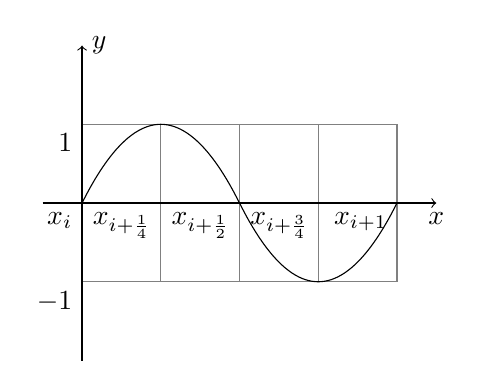
\begin{tikzpicture}[scale = 1]
	\draw[gray, step = 1cm] (0, -1) grid (4, 1);
	\draw[->] (-.5, 0) -- (4.5, 0);
	\draw[->] (0, -2) -- (0, 2);
	
	\node[anchor = north east] at (0, 0) {$ x_i $};
	\node[anchor = north east] at (1, 0) {$ x_{i+\frac{1}{4}} $};
	\node[anchor = north east] at (2, 0) {$ x_{i+\frac{1}{2}} $};
	\node[anchor = north east] at (3, 0) {$ x_{i+\frac{3}{4}} $};
	\node[anchor = north east] at (4, 0) {$ x_{i+1} $};
	\node[anchor = north east] at (0, 1) {$ 1 $};
	\node[anchor = north east] at (0, -1) {$ -1 $};
	\node[anchor = north] at (4.5, 0) {$ x $};
	\node[anchor = west] at (0, 2) {$ y $};
	
	
	\draw[domain = 0:2, smooth, variable=\x, black]
	plot ({\x}, {\x * (2-\x)})
	node[anchor = west] {};
	\draw[domain = 2:4, smooth, variable=\x, black]
	plot ({\x}, {-(4-\x) * (\x-2)})
	node[anchor = west] {};
	\end{tikzpicture}
\end{center}

We sum all the function on $[0,1]$,
\[
(I_{k+1}-I_k)(x^3) = 3\times2^{-3k-6}\sum_{i=0}^{2^k-1}(\varphi_{i+\frac{1}{4}}^{k+1} - \varphi_{i+\frac{3}{4}}^{k+1})
\]


\section{2D sparse grid for $xy$}
Consider the uniform gird $[0,1]^2$, and we define the grid
\[
T_k:(x_i,y_j),\quad x_i = ih,y_j = jh,\quad h = 2^{-k}
\]
$I_k$ is the piece linear interpolation operator which satisfies 
\[
(I_k f)(x_i,y_j) = f(x_i,y_j)
\]
We consider the grid $T_k$ and $T_{k-1}$. 
\begin{itemize}
	\item The basis functions on $T_{k-1}$ are $\varphi_1^{k-1},\varphi_2^{k-1},\varphi_3^{k-1}$.
	\item  The basis functions on refine grid $T_k$ are $\varphi_i^k,i=1,..,6$.
\end{itemize}
\begin{center}
	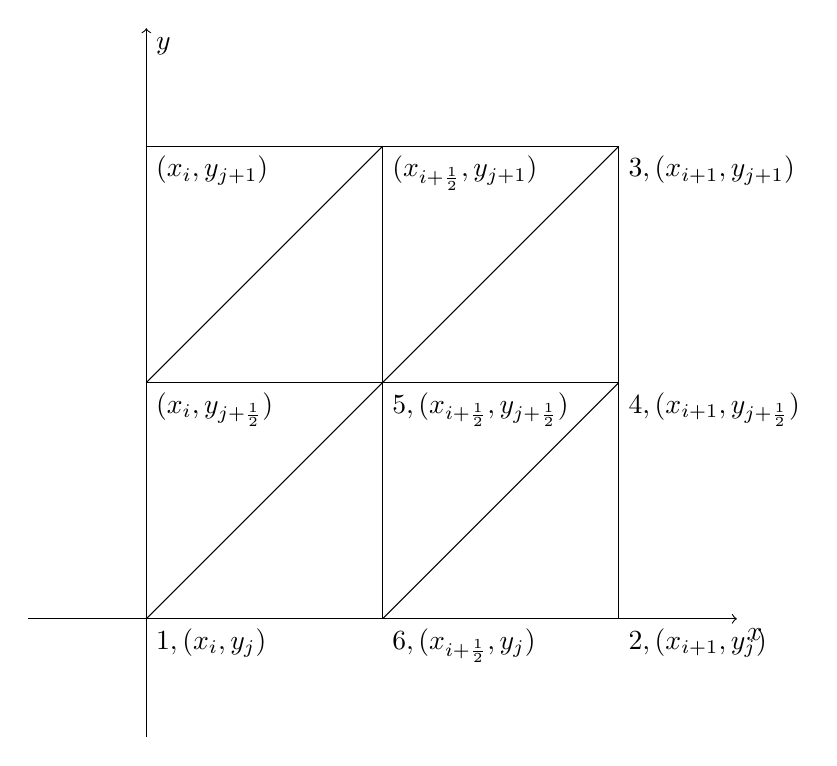
\begin{tikzpicture}[scale = 3 ]
	\draw[gray, step = 1cm] (0, 0) grid (2, 2);
	\draw[->] (-.5, 0) -- (2.5, 0);
	\draw[->] (0, -.5) -- (0, 2.5);
	\node[anchor = north west] at (0, 0) {$1, (x_i,y_j) $};
	\node[anchor = north west] at (2.5, 0) {$ x $};
	\node[anchor = north west] at (0, 2.5) {$ y $};
	\node[anchor = north west] at (1,0) {$6,(x_{i+\frac{1}{2}},y_j)$};
	\node[anchor = north west] at (2,0) {$2,(x_{i+1},y_j)$};
	\node[anchor = north west] at (0,1) {$(x_{i},y_{j+\frac{1}{2}})$};
	\node[anchor = north west] at (1,1) {$5,(x_{i+\frac{1}{2}},y_{j+\frac{1}{2}})$};
	\node[anchor = north west] at (2,1) {$4,(x_{i+1},y_{j+\frac{1}{2}})$};
	\node[anchor = north west] at (0,2) {$(x_{i},y_{j+1})$};
	\node[anchor = north west] at (1,2) {$(x_{i+\frac{1}{2}},y_{j+1})$};
	\node[anchor = north west] at (2,2) {$3,(x_{i+1},y_{j+1})$};
	
	\draw (0,0) -- (0,2);
	\draw (0,2) -- (2,2);
	\draw (2,2) -- (2,0);
	\draw (2,0) -- (0,0);
	\draw (0,0) -- (2,2);
	\draw (0,1) -- (1,2);
	\draw (1,0) -- (2,1);
	\draw (1,0) -- (1,2);
	\draw (0,1) -- (2,1);
	\end{tikzpicture}
\end{center}
\[
\begin{split}
I_{k-1}(xy) &= x_iy_j\varphi^{k-1}_1 + x_{i+1}y_j\varphi^{k-1}_2 + x_{i+1}y_{j+1}\varphi^{k-1}_3\\
&=x_iy_j(\varphi^k_1 + \frac{1}{2}(\varphi^k_5+\varphi^k_6)) + x_{i+1}y_j(\varphi^k_2 + \frac{1}{2}(\varphi^k_4+\varphi^k_6))\\
&+x_{i+1}y_{j+1}(\varphi^k_3+\frac{1}{2}(\varphi^k_4+\varphi^k_5))\\
&=x_iy_j\varphi^k_1 + x_{i+1}y_j\varphi^k_2+x_{i+1}y_{j+1}\varphi^k_3+\frac{1}{2}(x_{i+1}y_j+x_{i+1}y_{j+1})\varphi^k_4\\
&+\frac{1}{2}(x_{i}y_j+x_{i+1}y_{j+1})\varphi^k_5+\frac{1}{2}(x_{i}y_j+x_{i+1}y_{i})\varphi^k_6\\
&=x_iy_j\varphi^k_1 + x_{i+1}y_j\varphi^k_2+x_{i+1}y_{j+1}\varphi^k_3+x_{i+1}y_{j+\frac{1}{2}}\varphi^k_4\\
&+\frac{1}{2}(x_{i}y_j+x_{i+1}y_{j+1})\varphi^k_5+x_{i+\frac{1}{2}}y_j\varphi^k_6\\
I_k(xy) & = x_iy_j\varphi^k_1+x_{i+1}y_j\varphi^k_2+x_{i+1}y_{j+1}\varphi^k_3+x_{i+1}y_{j+\frac{1}{2}}\varphi^k_4 \\
&+x_{i+\frac{1}{2}}y_{j+\frac{1}{2}}\varphi^k_5 + x_{i+\frac{1}{2}}y_j\varphi^k_6
\end{split}
\]

Then,
\[
(I_k - I_{k-1})(xy) = (x_{i+\frac{1}{2}}y_{j+\frac{1}{2}}-\frac{1}{2}(x_{i}y_j+x_{i+1}y_{j+1}))\varphi^k_5 = -\frac{h^2}{4}\varphi_5^k
\]
The error is uniform! which is the basis function on each rectangle $[x_i,x_{i+1}]\times [y_j,y_{j+1}]$ and 
\[
\varphi_5^k(x_{i+\frac{1}{2}},y_{j+\frac{1}{2}}) = 1
\]


\section{Spectral approximation properties of ReLU DNN}
Here we will talk about how to use ReLU DNN to approximate polynomials
and then achieve the ``spectral" accuracy for analytical functions.
The main results can be found in \cite{yarotsky2017error},
\cite{wang2018exponential}. Some related works are
\cite{liang2016why,lu2017expressive}

First, we will introduce the following notation
\begin{itemize}
\item $x=(x_1,\ldots,x_d)$.
\item Colon notation for subscript: let $\{x_{m:n}\} = \{x_i:i = m,m+1,...,n\}$ and $\{x_{m_1:n_1,m_2:n_2}\}= \{x_{i,j}:i = m_1,...,n_1,j = m_2,...,n_2\}.$ 
\item Linear combination: denote $y\in \mathcal L(x_1,...,x_d)$ if
  there exist $\beta_i\in \mathbb{R},i=1,...,d,$ such that $y =
  \beta_0+\beta_1x_1+\cdots+\beta_d x_d$.
\item Linear combination with ReLU activation: denote $\tilde{y}\in
  \tilde{\mathcal L}(x_1,...,x_d)$ if there exists $y\in
  \mathcal{L}(x_1,...,x_d)$ and $\tilde{y} = \mbox{ReLU}(y) =
  \max(y,0).$
\item $\tilde {\mathcal L} =\sigma\circ\mathcal L$
\end{itemize}
\begin{definition}
Given a function $f(x)$, if there exist variables $\{y_{1:L,1:M}\}$ such that 
\begin{equation}
y_{1,m}\in \tilde{\mathcal L}(x),\quad y_{l+1,m} \in \tilde{\mathcal L}(x,y_{l,1:M}),\quad f\in\mathcal{L}(x,y_{1:L,1:M}),
\end{equation}\label{def:netclass}
where $m=1,...,M,l=1,...,L-1$, then $f$ is said to be in the neural nets class $\mathcal{F}_{L,M}(\mathbb{R}^d)$, and $\{y_{1:L,1:M}\}$ is called a set of hidden variables of $f$. 
\end{definition}
\newpage
%\begin{properties}
\begin{proposition}
A function $f\in \mathcal F_{L,M}(\mathbb R^d)$ can be represented by a ReLU network with depth $L+1$ and width $M+d+1$.
\end{proposition}
%\end{properties}
\begin{proof}
Let $\{y_{1:L}\}$ be the hidden variables of $f$ that satisfies (\ref{def:netclass}), where
$$
f = \alpha_0 + \sum_{i=1}^d \alpha_ix_i+\sum_{l=1}^L\sum_{m=1}^M \beta_{l,m}y_{l,m}.
$$
$$
h\leftarrow (y,ex^T), e=(1,\ldots 1)^T.
$$
Consider the following variables $\{h_{1:L,1:M}\}$:
$$
h_{l,1:M} = y_{l,1:M}, \quad h_{l,M+1:M+d} = x_{1:d}
$$
for $l = 1,...,L,$ and
$$
h_{1,M+d+1} = \alpha_0 + \sum_{i=1}^d\alpha_ix_i,\quad h_{l+1,M+d+1} =h_{l,M+d+1} + \sum_{m=1}^M\beta_{l,m}h_{l,m}
$$
for $l=1,...,L-1$. One can see that $h_{1,m}\in \tilde{\mathcal L}(x),h_{l+1,m}\in \tilde{L}(h_{l,1:M+d+1}),m = 1,...,M+d+1,l = 1,...,L-1,$ and $f\in \mathcal{L}(h_{L,1:M+d+1}),$ which is a representation of a standard neural net.
\end{proof}

%\begin{properties}
\begin{proposition}\label{prop:net class}
(Addition and composition of neural net class $\mathcal F_{L,M}$)
\begin{itemize}
\item[1]
$$
\mathcal F_{L_1,M} + \mathcal{F}_{L_2,M} \subseteq \mathcal{F}_{L_1+L_2,M},
$$
i.e. if $f_1\in \mathcal F_{L_1,M}(\mathbb{R}^d)$ and $f_2\in \mathcal{F}_{L_2,M}(\mathbb{R}^d),$ then $f_1+f_2\in\mathcal{F}_{L_1+L_2,M}(\mathbb{R}^d)$.
\item[2]
$$
\mathcal F_{L_2,M}\circ \mathcal F_{L_1,M+1} \subseteq \mathcal F_{L_1+L_2,M+1}.
$$ 
i.e. if $f_1(x)\in \mathcal{F}_{L_1,M+1}(\mathbb{R}^d)$ and $f_2(x_0,x)\in \mathcal{F}_{L_2,M}(\mathbb{R}^{d+1}),$ then 
$$
f_2(f_1(x),x)\in \mathcal{F}_{L_1+L_2,M+1}(\mathbb{R}^d).
$$
\end{itemize}
\end{proposition}
%\end{properties}

\newpage
\begin{proof}
For the addition property, denote the hidden variables of $f_1$ and $f_2$ as $\{y_{1:L_1,1:M}^{(1)}\}$ and $\{y_{1:L_2,1:M}^{(2)}\}$. 
So we have 
\[
f_1 = \alpha_0^1 + \sum_{i=1}^d \alpha^1_ix_i+\sum_{l=1}^L\sum_{m=1}^M \beta^1_{l,m}y^{(1)}_{l,m}
\]
\[
f_2 = \alpha_0^2 + \sum_{i=1}^d \alpha^2_ix_i+\sum_{l=1}^L\sum_{m=1}^M \beta^2_{l,m}y^{(2)}_{l,m}
\]
\[
f_1+f_2 = \alpha_0^1 + \alpha_0^2 + \sum_{i=1}^d (\alpha_i^1+\alpha_i^2)x_i + \sum_{l=1}^L\sum_{m=1}^M \beta^1_{l,m}y^{(1)}_{l,m} +\sum_{l=1}^L\sum_{m=1}^M \beta^2_{l,m}y^{(2)}_{l,m}
\]
$$
y^{(1)}_{1,1:M} = \sigma\circ \mathcal{L}(x),y^{(1)}_{2,1:M} = \sigma\circ \mathcal L(x,y^{(1)}_{1,1:M}),\cdots,y^{(1)}_{L_1,1:M}=\sigma\circ \mathcal L(x,y^{(1)}_{L_1-1,1:M}),
$$
$$
y^{(2)}_{1,1:M} = \sigma\circ \mathcal{L}(x) =\sigma(\mathcal L(x)+\bm 0\cdot y^{(1)}_{L_1,1:M}) = \sigma\circ \mathcal{L}(x,y^{(1)}_{L_1,1:M})
$$
$$
y^{(2)}_{2,1:M} = \sigma\circ \mathcal L(x,y^{(2)}_{1,1:M}),\cdots,y^{(2)}_{L_2,1:M}=\sigma\circ \mathcal L(x,y^{(2)}_{L_2-1,1:M}),
$$
so $f_1 + f_2 \in \mathcal{F}_{L_1+L_2,M}$
Let
$$
y_{1:L_1,1:M} = y_{1:L_1,1:M}^{(1)},\quad y_{L_1+1:L_1+L_2,1:M} = y_{1:L_2,1:M}^{(2)}. 
$$
By definition, $\{y_{1:L_1+L_2,1:M}\}$ is a set of hidden variables of $f_1+f_2$. Thus $f_1+f_2\in \mathcal F_{L_1+L_2,M}.$

For the composition property, let the hidden variables of $f_1$ and $f_1$ as $\{y_{1:L_1,1:M+1}^{(1)}\}$ and $\{y_{1:L_2,1:M}^{(2)}\}$. Let
$$
y_{1:L_1,1:M+1} = y_{1:L_1,1:M+1}^{(1)},\quad y_{L_1+1:L_1+L_2,1:M} = y_{1:L_2,1:M}^{(2)},
$$
$$
y_{L_1+1,M+1} =\cdots= y_{L_1+L_2,M+1} = f_1(x).
$$
One can see that $\{y_{1:L_1+L_2,1:M+1}\}$ is a set of hidden variables of $f_2(f_1(\bm x),\bm x)$, thus the composition property holds.
\end{proof}

\begin{definition}
Given a continuous function $\varphi(\bm{x}),\bm{x} \in [-1,1]^d$ and a continuous function class $\mathcal F([-1,1]^d),$ define the $L^\infty$ distance
$$
\mbox{dist} (\varphi,\mathcal F) = \inf_{f\in \mathcal F} \max_{\bm x \in [-1,1]^d} |\varphi(\bm{x}) - f(\bm{x})|.
$$
\end{definition}

%\begin{properties}
\begin{proposition}\label{prop:dis}
(Addition and composition properties for distance function)
\begin{itemize}
\item[1] Let $\varphi_1$ and $\varphi_2$ be continuous functions. Let $\mathcal F_{1}$ and $\mathcal F_2$ be two continuous function classes, then 
$$
\mbox{dist}(\alpha_{1}\varphi_1+\alpha_{2}\varphi_2,\mathcal{F}_1+\mathcal F_2)\le |\alpha_1|\mbox{dist}(\varphi_1,\mathcal F_1) + |\alpha_2|\mbox{dist}(\varphi_2,\mathcal F_2),
$$
where $\alpha_1$ and $\alpha_2$ are two real numbers.
\item[2] Assume that $\varphi_1(\bm x) = \varphi_1(x_1,...,x_d),\varphi_2(y,\bm x) = \varphi_2(y,x_1,...,x_d)$ satisfy $\varphi_1([-1,1]^d)\subseteq[-1,1]$. Let $\mathcal F_1([-1,1]^d),\mathcal F_2([-1,1]^{d+1})$ be two continuous function classes, then
$$
\mbox{dist}(\varphi_2(\varphi_1(\bm x),\bm x),\mathcal F_2\circ \mathcal F_1)\le L_{\varphi_2}\mbox{dist}(\varphi_1,\mathcal F_1) +\mbox{dist}(\varphi_2,\mathcal F_2)
$$
where $L_{\varphi_2}$ is the Lipschitz norm of $\varphi_2$ with respect to $y$.
\end{itemize}
\end{proposition}
%\end{properties}
\begin{proof}
The additional property obviously holds. Now we prove the composition property. For any $f_1\in\mathcal F_1,f_2\in \mathcal F_2$, one has
\[
\begin{split}
|\varphi_2(\varphi_1(\bm x),\bm x) - f_2(f_1(\bm x),\bm x)|&\le |\varphi_2(\varphi_1(\bm x),\bm x) - \varphi_2(f_1(\bm x),\bm x)|+|\varphi_2(f_1(\bm x),\bm x)-f_2(f_1(\bm x),\bm x)|\\
& \le L_{\varphi_2} ||\varphi_1(\bm x) -f_1(\bm x)||_\infty +||\varphi_2(y,\bm x) - f_2(y,\bm x)||_\infty
\end{split}
\]
Take $f_1^* = \argmin_f ||\varphi_1(\bm x) - f(\bm x)||_\infty$ and $f_2^* = \argmin_f ||\varphi_2(y,\bm x) - f(y,\bm x)||_\infty$, then it is proved.
\end{proof}

\begin{lemma}\label{lem:xsquare}
The function $\varphi(x) = x^2,x\in [-1,1]$ can be approximated by deep neural nets with an exponential convergence rate:
$$
\mbox{dist}(x^2,\mathcal{F}_{L,2}([-1,1]))\le 2^{-2L}.
$$
\end{lemma}
\begin{proof}
Consider the function
$$
g(y) = \left\{\begin{split}
	&2y,&\quad 0\le y<1/2,\\
	&2(1-y),&\quad 1/2\le y\le 1,
	\end{split}\right.
$$
then 
\begin{equation}\label{func:g}
g(y) = 2y -4\mbox{ReLU}(y-1/2)
\end{equation}
in $[0,1]$. Define the hidden variables $\{y_{1:L,1:2}\}$ as follows:
\[
\begin{split}
 y_{1,1} = \mbox{ReLU}(x),&\quad y_{1,2}=\mbox{ReLU}(-x),\\
 y_{2,1} = \mbox{ReLU}(y_{1,1}+y_{1,2}),&\quad y_{2,2} = \mbox{ReLU}(y_{1,1}+y_{1,2}-1/2),\\
 y_{2,1} = \mbox{ReLU}(|x|),&\quad y_{2,2} = \mbox{ReLU}(|x|-1/2),\\
 y_{l+1,1} = \mbox{ReLU}(2y_{l,1}-4y_{l,2}),&\quad y_{l+1,2} = \mbox{ReLU}(2y_{l,1}-4y_{l,2}-1/2)\\
\end{split}
\]
for $l = 2,3,...,L-1$. Using induction, one can see that $|x| = y_{1,1}+y_{1,2}$ and 
\begin{equation}\label{func:glinduction}
g_l(|x|)=\underbrace{g\circ g\circ \cdots \circ g}_{l}(|x|) = 2y_{l+1,1}-4y_{l+1,2},\quad l=1,...,L-1,
\end{equation} 
for $x\in [-1,1]$. i.e.
\[
\begin{split}
g_l(|x|) &= g\left(g_{l-1}(|x|)\right)\\
         &= g(2y_{l,1}-4y_{l,2})\qquad (\mbox{Eq~(\ref{func:g})})\\
         &= 2(2y_{l,1}-4y_{l,2}) - 4\mbox{ReLU}(2y_{l,1}-4y_{l,2}-1/2)\qquad (g_{l-1}(|x|)\ge 0~\mbox{if}~x\in[0,1])\\
         &= 2\mbox{ReLU}(2y_{l,1}-4y_{l,2})- 4\mbox{ReLU}(2y_{l,1}-4y_{l,2}-1/2)\\
         & = 2y_{l+1,1} - 4y_{l+1,2}\\
\end{split}
\]
by induction, Eq (\ref{func:glinduction}) holds.
\begin{figure}[h]
	\centering
	\includegraphics[width=0.8\textwidth]{figures/dl_approx_analytic_gl}
	\caption{The figure of $g_l(x)$}
	\label{fig:gl}
\end{figure}

Let $f_m$ be the piecewise linear interpolation of $f$ with $2^m+1$ uniformly distributed breakpoints $\frac{k}{2^m},k = 0,...,2^m:$
$$
f_{m}(\frac{k}{2^m}) = (\frac{k}{2^m})^2,\quad k = 0,...,2^m.
$$
Note that refining the interpolation from $f_{m-1}$ to $f_m$ amounts to adjusting it by a function proportional to a sawtooth function:
$$
f_{m-1}(x) - f_m(x) = \frac{g_m(x)}{2^{2m}}.
$$
Hence 
$$
f_{L-1}(|x|) = |x| - \sum_{l=1}^{L-1}\frac{g_l(|x|)}{2^{2l}} .
$$
then $f_{L-1}\in \mathcal{F}_{L,2}$, and 
\[
\begin{split}
||x^2-f_{L-1}(x)||_{\infty} & = \max_{k} \max_{x\in [\frac{k}{2^{L-1}},\frac{k+1}{2^{L-1}}]} |x^2 - f_{L-1}(x)|\\
  & = \max_{k} |(\frac{1}{2}(\frac{k}{2^{L-1}}+\frac{k+1}{2^{L-1}}))^2 - f_{L-1}(\frac{1}{2}(\frac{k}{2^{L-1}}+\frac{k+1}{2^{L-1}}))|\\
  & = \max_k |(\frac{1}{2}(\frac{k}{2^{L-1}}+\frac{k+1}{2^{L-1}}))^2 - \frac{1}{2}((\frac{k}{2^{L-1}})^2+(\frac{k+1}{2^{L-1}})^2))|\\
  &=\frac{1}{4^L}.
\end{split}
\]
$|x^2-f_{L-1}(x)|\le 2^{-2L}$ for $x\in[-1,1].$
\end{proof}

\begin{lemma}\label{lem:xy}
For multiplication function $\varphi(x,y) = xy$, we have 
$$
\mbox{dist}(xy,\mathcal{F}_{3L,2}([-1,1]^2))\le 3\cdot 2^{-2L}.
$$
\begin{proof}
Notice that
$$
\varphi = xy = 2\left(\frac{x+y}{2} \right)^2-\frac{1}{2}x^2-\frac{1}{2}y^2.
$$
\[
\begin{split}
\mbox{dist}(xy,\mathcal{F}_{3L,2}([-1,1]^d))&\le2\mbox{dist}(\left(\frac{x+y}{2} \right)^2,\mathcal{F}_{L,2}([-1,1]^2)) + \frac{1}{2} \mbox{dist}(x^2,\mathcal{F}_{L,2}([-1,1]^2)) \\
 &+\frac{1}{2} \mbox{dist}(y^2,\mathcal{F}_{L,2}([-1,1]^2))\\
 &\le 3\mbox{dist}(x^2,\mathcal{F}_{L,2}([-1,1]^2))\\
 &\le 3\mbox{dist}(x^2,\mathcal{F}_{L,2}([-1,1])) + \mbox{dist}(I_x,\mathcal{F}_{L,2}([-1,1]^2))\\
 &= 3\cdot 2^{-2L}
\end{split}
\]
\end{proof}
\end{lemma}

\begin{lemma}
For a monomial $M_p(\bm x)$ of $d$ variables with degree $p$, we have
$$
\mbox{dist}(M_p,\mathcal F_{3(p-1)L,3}(\mathbb R^d))\le 3(p-1)\cdot 2^{-2L}.
$$
\end{lemma}

\begin{proof}
Let $M_p(\bm x)=x_{i_1}x_{i_2}\cdots x_{i_p},i_1,...,i_p\in\{1,...,d\}.$ Using induction, assume that the lemma holds for the degree-$p$ monomial $M_p$, consider a degree-$(p+1)$ monomial $M_{p+1}(\bm{x}) = M_p(\bm{x})\cdot x_{i_{p+1}}$. Let $\varphi(y,x) = yx,$ then $M_{p+1}(\bm x) = \varphi(M_p(\bm{x}),x_{i_{p+1}})$. We have
\[
\begin{split}
\mbox{dist}(M_{p+1},\mathcal{F}_{3pL,3})&\le \mbox{dist}(\varphi(M_p(\bm x),x_{i_{p+1}}),\mathcal F_{3L,2}\circ \mathcal F_{3(p-1)L,3})\\
& \le L_{\varphi}\mbox{dist}(M_p,\mathcal{F}_{3(p-1)L,3})+\mbox{dist}(\varphi,\mathcal F_{3L,2})\le 3p\cdot 2^{-2L}.
\end{split}
\]
Note that the Lipschitz norm $L_{\varphi}=1$ since $x_{i_{p+1}}\in [-1,1].$
\end{proof}

\begin{lemma}
For a degree-$p$ polynomial $P_p(\bm{x}) = \sum_{|\bm{k}|\le p}a_{\bm k}\bm x^{\bm k},\bm x\in [-1,1]^d,\bm k = (k_1,...,k_d)\in\mathbb{N}^d,$ we have 
\[
\mbox{dist}\left(P_p,\mathcal F_{\binom{p+d}{d}(p-1)L,3}\right)<3(p-1)\cdot 2^{-2L}\sum_{|\bm k|\le p}|a_{\bm k}|
\]
\end{lemma}\label{lem:poly}

\begin{proof}
This lemma can be proved by the properties \ref{prop:net class}, \ref{prop:dis} and lemma \ref{lem:poly}.
Note that the number of monomials of $d$ variables with degree less or equal to $p$ is $\binom{p+d}{d}$.
$$
k_1 + k_2 + \cdots + k_d \le p,
$$
Add a variable $k_{d+1}$, we have
$$
k_1 + k_2 + \cdots + k_d + k_{d+1} = p.
$$
the number of the non-negative solution is $\binom{p+d}{d}$.
\end{proof}

\begin{theorem}
Let $f$ be an analytic function over $(-1,1)^d$. Assume that the power series $f(\bm x) = \sum_{\bm k\in \mathbb N^d}a_{\bm k}\bm x^{\bm k}$ is absolutely convergent in $[-1,1]^d.$ Then for any $\delta>0,$ there exists a function $\hat f$ that can be represented by a deep ReLU network with depth $L$ and width $d+4$, such that
\[
|f(\bm x) - \hat f(\bm x)|<2\sum_{\bm k\in \mathbb N^d}|a_{\bm k}|\cdot \exp\left(-d\delta\left(e^{-1}L^{1/2d}-1\right)\right)
\]
for all $\bm x\in [-1+\delta,1-\delta]^d.$
\end{theorem}
\begin{proof}
Let $\epsilon = \exp(-d\delta(e^{-1}L^{1/2d}-1)),$ then $L = [e(\frac{1}{d\delta}\log\frac{1}{\epsilon}+1)]^{2d}$. Without loss of generality, assume $\sum_{\bm k}|a_{\bm k}|=1.$ We will show that there exists $\hat f\in \mathcal F_{L,3}$ such that $||f-\hat f||_{\infty}<2\epsilon.$
Denote 
$$
f(\bm x) = P_p(\bm x) + R(\bm x): = \sum_{|\bm k|\le p}a_{\bm k}\bm x^{\bm k} +  \sum_{|\bm k|> p}a_{\bm k}\bm x^{\bm k}.
$$
For $\bm x\in [-1+\delta,1-\delta]^d$, we have $|R(\bm x)|<(1-\delta)^p$, thus truncation to $p = \frac{1}{\delta}\log\frac{1}{\epsilon}$ with ensure $|R(\bm x)|<2\epsilon$. From lemma \ref{lem:poly}, we have dist$(P_p,\mathcal F_{L,3})<3(p-1)\cdot 2^{-2L'}$, where 
\[
\begin{split}
L' &= L\binom{p+d}{d}^{-1}(p-1)^{-1}\\
   &\ge L(\frac{(p+d)!}{p!d!})^{-1}p^{-1}\quad (d! \thicksim \sqrt{2\pi d}(d/e)^d)\\
   &\ge L(\frac{(p+d)^d}{(d/e)^d})^{-1}p^{-1}\\
   &= L[e(\frac{1}{d\delta}\log \frac{1}{\epsilon}+1)]^{-d}(\frac{1}{\delta}\log\frac{1}{\epsilon})^{-1}\\
   & = [e(\frac{1}{d\delta}\log \frac{1}{\epsilon}+1)]^{d}(\frac{1}{\delta}\log\frac{1}{\epsilon})^{-1}\\
   & \ge e^d (\frac{1}{\delta}\log\frac{1}{\epsilon}) \\
   &\gg\log\frac{1}{\delta}+ \log\frac{1}{\epsilon}
\end{split}
\]
for $d\ge 2$ and $\epsilon\ll 1$, then dist$(P_p,\mathcal F_{L,3})<3(p-1)\cdot 2^{-2L'} = 3(p-1)(\epsilon^2+\delta^2)\ll\epsilon$. Thus there exists $\hat f\in \mathcal F_{L,3}$ such that $||P_p - \hat f||_{\infty}<\epsilon$, and $||f-\hat f||_{\infty}\le ||f-P_p||_\infty + ||P_p - \hat f||_\infty<3\epsilon$.
\end{proof}

\subsection{Cosine Function}

Let $f(\bm x) = \cos(|\bm x|^2)$. Assume that the power series 
\[
f(\bm x) = \sum_{k=0}^{+\infty} \frac{(-1)^k|\bm x|^{4k}}{(2k)!},\quad \bm x\in [-1,1]^d.
\]
Denote
\[
\begin{split}
f(\bm x) = P_p(\bm x) + R(\bm x): &= \sum_{|\bm k|\le p}a_{\bm k} \bm x^{\bm k} + \sum_{|\bm k|>p} a_{\bm k} \bm x^{\bm k}\\
&=\sum_{k\le p} \frac{(-1)^k}{(2k)!}|\bm x|^{4 k} + \frac{(-1)^{p+1}}{(2(p+1))!}|\bm t|^{4 (p+1)},\quad \bm t\in[0,1]^d\\
\end{split}
\]


Let $p(\varepsilon,d)=p$ be large, s.t.
\[
\big|\frac{(-1)^{p+1}}{(2(p+1))!}|\bm t|^{4(p+1)}\big| < \varepsilon.
\]
\[
\begin{split}
\big|\frac{(-1)^{p+1}}{(2(p+1))!}|\bm t|^{4 (p+1)}\big| &\le \frac{d^{2(p+1)}}{(2(p+1))!}\\
& \le C(\frac{ed}{2(p+1)})^{2(p+1)}\\
\end{split}
\]
Let $p = \log \frac{1}{\varepsilon}-1$, then 
\[
(\frac{ed}{2(p+1)})^{2(p+1)}\le (\frac{ed}{2\log \frac{1}{\varepsilon}})^{2\log\frac{1}{\varepsilon}}\le \varepsilon^{-2\log \frac{ed}{2\log \frac{1}{\varepsilon}}}\le \varepsilon
\]

We want to show that 
\[
\mbox{dist}(P_{p(\varepsilon,d)},\mathcal{F}_{L(\varepsilon,d),3})<\varepsilon.
\]

By Lemma~\ref{lem:poly}, we have 
\[
\begin{split}
\mbox{dist}(P_{p},\mathcal{F}_{L,3})&<3(p-1)2^{-\frac{2L}{\binom{p+d}{d}(p-1)}}\sum_{\bm k\le p}|a_{\bm k}|\\
&\le3p2^{-\frac{2Ld^d}{p(p+d)^de^d}}\sum_{|\bm k|\le p}|a_{\bm k}|.
\end{split}
\]

Let $L = \frac{1}{2} ((p+d)e/d)^{2d}$, we can see that
\[
\begin{split}
\mbox{dist}(P_{p},\mathcal{F}_{L,3})
&\le3p2^{-\frac{2Ld^d}{p(p+d)^de^d}}\sum_{|\bm k|\le p}|a_{\bm k}|\\
&= 3p2^{-\frac{(p+d)^de^d}{d^dp}}\sum_{|\bm k|\le p}|a_{\bm k}|\\
&\le 3(\log \frac{1}{\varepsilon}-1)2^{-\frac{e^d}{4}(d-1)d(\log \frac{1}{\varepsilon}-1)} \sum_{|\bm k|\le p}|a_{\bm k}|\\
&\le C(d)\varepsilon^{\frac{e^d}{4}d(d-1)\log 2}\log\frac{1}{\varepsilon}\le \varepsilon
\end{split}
\]

Take 
\[
\varepsilon = \exp\left(-d\left(e^{-1}(2L)^{1/2d}-1\right)-1\right)
\]
then, we have 
\[
\mbox{dist}(f,\mathcal{F}_{L,3})\le\mbox{dist}(P_{p},\mathcal{F}_{L,3})+ R(\bm x) \le 2\varepsilon \le 2e^{-d\left(e^{-1}(2L)^{1/2d}-1\right)-1}
\]



\section{A modified ResNet structure and its properties}
Using the notation in Lin Li's notes, we have the next two properties for this modified ResNet structure in $\mathbb{R}^d$ as
\begin{itemize}
	\item Added with depth
	$$
	\mathcal F_{L_1,M}(\mathbb{R}^d) + \mathcal{F}_{L_2,M}(\mathbb{R}^d)  \subseteq \mathcal{F}_{L_1+L_2,M}(\mathbb{R}^d) .
	$$
	\item Added with width 
	$$
	\mathcal F_{L,M_1}(\mathbb{R}^d)  + \mathcal{F}_{L,M_2}(\mathbb{R}^d)  \subseteq \mathcal{F}_{L,M_1 + M_2}(\mathbb{R}^d) .
	$$
\end{itemize}
This second property works for all DNN structures, but the first structure only works for this special ResNet structure with any activation functions.

\section{h-method by partition of unit}
First, for any positive integer $M$, let us consider the next partition of unit function of $[0, 1]^d$
$$
\phi_{\bm m}(x) = \prod_{k=1}^d \Phi\left(3M(x_k - \frac{m_k}{M})\right),
$$
with 
$$
{\bm m} = (m_1, m_2, \cdots, m_d) \in \{0,1, \cdots,M\}^d = \mathcal{M},
$$
and 
$$
\Phi(x) = \begin{cases}
1, \quad  &|x| \le 1, \\
0, \quad &|x| \ge 2, \\
2 - |x|, \quad &1 < |x| <2.
\end{cases}
$$
Thus, we have
$$
\sum_{{\bm m} \in \mathcal{M}} \phi_{\bm m}({\bm x}) = 1, \quad \forall {\bm x} \in [0,1]^d.
$$

\begin{itemize}
	\item How to choose M?
\end{itemize}
\section{p-method by local Taylor expansion}
Taylor expansion with $p-$th polynomials at most at ${\bm x} = \frac{{\bm m}}{M}$:
$$
P_{{\bm m}, p}({\bm x}) = \sum_{|{\bm n}| < p}\frac{\partial^{\bm n}f}{ \bm n !}\left(\frac{{\bm m}}{M}\right) ({\bm x} - \frac{{\bm m}}{M})^{\bm n}.
$$
Here we just consider about the local Taylor expansion, so the global approximation function is
$$
f_p({\bm x}) = \sum_{{\bm m} \in \mathcal{M}} \phi_{\bm m} P_{{\bm m}, p}({\bm x}), \quad \forall {\bm x} \in [0,1]^d.
$$

\begin{itemize}
	\item How to choose $p$? Balance with the residual term?
\end{itemize}

\section{Error estimate for $|f - f_p|_{0,\infty}$}
\begin{align*}\label{fperoor}
|f - f_p|_{0,\infty} &= |\sum_{\bm m} \phi_{\bm m}(f - P_{{\bm m}, p})|_{0, \infty},  \\
&\le \max_{{\bm m} \in \mathcal{M}}  |\sum_{\bm m} \phi_{\bm m}(f - P_{{\bm m}, p})|_{0, \infty,  |{\bm x} - \frac{\bm m}{M}| \le {\frac{1}{M}}}, \\
&\le \max_{{\bm m} \in \mathcal{M}} \sum_{ {\bm m} \in \mathcal{N}({\bm m})} |f - P_{{\bm m}, p}|_{0,\infty, |{\bm x} - \frac{\bm m}{M}| \le {\frac{1}{M}}}, \\
&\le \max_{{\bm m} \in \mathcal{M}}  2^d \max_{{\bm m} \in \mathcal{N}({\bm m})} |f - P_{{\bm m}, p}|_{0,\infty, |{\bm x} - \frac{\bm m}{M}| \le {\frac{1}{M}}}, \\
&\le \left( 2^{d} \left( \frac{1}{M} \right)^p \frac{d^p}{ p!} \right)|f|_{p, \infty}.
\end{align*}

\section{Approximate $f_p$ by ReLU DNN with error estimate}
\subsection{Approximate $\phi_m P_{m, p}$}
\begin{itemize}
	\item Approximate $\phi_{\bm m}$ 
	
	First we know that 
	$$
	\Phi(x) = ReLU(x+2) - ReLU(x+1) - ReLU(x-1) + ReLU(x-2),
	$$ 
	so 
	$$
	\inf_{v \in DNN_{J}} |\phi_{\bm m} - v| \le 2^{-\frac{2J}{3d}}.
	$$
	\item Approximate $P_{{\bm m}, p}$ (Original version in Yarotsky2017 )
	
	Assume that 
	$$
	P_{{\bm m}, p} = \sum_{|{\bm n}| \le p}a_{\bm m, \bm n} {(\bm x - \frac{\bm m}{M})}^{\bm n},
	$$
	then 
	$$
	\inf_{v \in DNN^{T}_{J}} |P_{{\bm m}, p} - v| \le (\max_{ \bm n} a_{\bm m,\bm n})2^{-\frac{2J}{3(p-1)}},
	$$
	with 
	$$
	T = \tbinom{p+d}{d}(d+4).
	$$
	
	\item Approximate $\phi_{\bm m} P_{\bm m, p}$
	$$
	\inf_{v \in DNN^{T}_{J}} |\phi_{\bm m} P_{\bm m, p} - v| \le (\max_{ \bm n} a_{\bm m,\bm n}) \max\{2^{-\frac{2J}{9(p-1)}},  2^{-\frac{2J}{9d}}\},
	$$
\end{itemize}

\begin{remark}
In fact, in Yarotsky2017 they estimate as:
$$
\inf_{v \in DNN^{T}_{J}} |\phi_{\bm m} P_{\bm m, p} - v| \le (\max_{ \bm n} a_{\bm m,\bm n}) 2^{-\frac{2J}{9(p + d -1)}},
$$	
and 
$$
\max_{ \bm n} a_{\bm m,\bm n} \le 1,
$$
for 
$$
\|f\|_{p+1,\infty} \le 1.
$$
\end{remark}


\subsection{Approximate $f_p$}
In Yarotsky2017, 
$$
\inf_{v \in DNN^{\hat T}_{J}} |f_p - v| \le (\max_{ \bm n} a_{\bm m,\bm n}) 2^d d^p2^{-\frac{2J}{9(p + d -1)}},
$$
with 
$$
\hat T = d^p (M+1)^d.
$$

\begin{remark}
	Here is a difference in Yarotsky2017 and Prof. E's paper: 
	\begin{itemize}
		\item In Prof. E's paper
		$$
		\sum_{k} a_k e_k \le \max_k e_k (\sum_k a_k).
		$$
		\item In Yarotsky2017
		$$
		\sum_{k} a_k e_k \le \max_k a_k (\sum_k e_k).
		$$
	\end{itemize}
\end{remark}
More exactly, we can get
\begin{align}
\inf_{v \in DNN^{T}_{J}} |f_p - v| &\le  2^d (p+d) \sum_{k=0}^{p-1}\sum_{|\bm n|=k} a_{\bm m, \bm n}2^{-\frac{2J}{3(p + d )}}, \\
&\le  2^d (p+d) 2^{-\frac{2J}{3(p + d )}} \left(\sum_{k=0}^{p-1}\sum_{|\bm n|=k} \frac{C(\bm n)}{k!} |f|_{k,\infty}\right), \\
&= 2^d (p+d) 2^{-\frac{2J}{3(p + d )}} \left(\sum_{k=0}^{p-1}\sum_{|\bm n|=k} \frac{d^k}{k!} \right)\|f\|_{p-1,\infty}, \\
&\le  2^d (p+d) e^d 2^{-\frac{2J}{3(p + d )}}\|f\|_{p-1,\infty}. 
\end{align}


\section{Balance $m, p$ with error and depth(d.o.f)}
In the end, we have
\begin{align}
\|f- \tilde f_p\|_{0,\infty} &\le \|f - f_p\|_{0,\infty} + \|f_p - \tilde f_p\|_{0,\infty}, \\
&\le \left[ \frac{2^dd^p}{p!}(\frac{1}{M})^p + 2^d e^d (d+p) 2^{-\frac{2J}{3(d+p)}}\right] \|f\|_{p, \infty}
\end{align}

Question: How to balance $m,p$? 

The d.o.f of above model is about 
$$
N = (M+1)^d \tbinom{p+d}{d} d^2 J,
$$
so the result for the approximation w.r.t the d.o.f is
\begin{align}
\|f- \tilde f_p\|_{0,\infty} &\le \|f - f_p\|_{0,\infty} + \|f_p - \tilde f_p\|_{0,\infty}, \\
&\le \left[ \frac{2^dd^p}{p!}(\frac{1}{M})^p + 2^d e^d (d+p) 2^{-\frac{2N}{3(d+p)(M+1)^d \tbinom{p+d}{d}d^2}}\right] \|f\|_{p, \infty}.
\end{align}

There are some problems to balance this two terms.

\subsection{Exponential convergence in this case}
Take $M = 2$, and 
$$
p = \log_2\frac{1}{\epsilon}
$$
and $\epsilon << 1$ such that 
$$
\frac{2^dd^p}{p!} \le 1,
$$
then we can take 
$$
N = \left( 3e(1 + \frac{p}{d})\right)^{2d},
$$
then it is easy to see
$$
\|f- \tilde f_p\|_{0,\infty} \le 2\epsilon \lesssim \exp({ -d((3e)^{-1}N^{\frac{1}{2d}} - 1)}).
$$
\begin{proof}\label{proof:1}
\begin{align}
-\frac{2N}{3(d+p)(M+1)^d \tbinom{p+d}{d}d^2} &\le\frac{-2(3e(1+\frac{p}{d}))^d}{3(p+d)d^2}, \\
&\le -\frac{2e}{3}\times \frac{3^d e^{d-1}(\tbinom{d}{2}\frac{p^2}{d^2} + p)}{pd^3}, \quad (d \ge 2) \\
&= -\left( \frac{3^de^{d-1}(d-1)}{2d^2}p + \frac{3^de^{d-1}}{d^3} \right), \\
&\le - \left((\log_2{e}) p + (1+\log_2e)d\right). \quad (d \ge 2)
\end{align}
\end{proof}

\begin{remark}
	In Prof. E's result, it is:
	\begin{align}
	\|f- \tilde f_p\|_{0,\infty, I_\delta^d} &\le \|f - f_p\|_{0,\infty, I_\delta^d} + \|f_p - \tilde f_p\|_{0,\infty, I_\delta^d}, \\
	&\le \min_{p} \left[(1-\delta)^p + 3p2^{-\frac{2J}{3pd^2\tbinom{p+d}{d}}}\right] (\sum_{\bm n}a_{\bm n}).
	\end{align}
	seems easier to balance.
	\end{remark}

\section{Just $p$ version: expansion at $ (\frac{1}{2}, \cdots, \frac{1}{2})$}

For $\Omega = [0,1]^d$, and $f_p$ is like
$$
f_p = \sum_{k=0}^{p-1} \frac{1}{k!} \left(\sum_{i=1}^d (x_i - \frac{1}{2})\frac{\partial}{\partial x^i}\right)^k f |_{x = \frac{\bm 1}{\bm 2}},
$$
then we have:
\begin{align}
\|f - f_p\|_{0, \infty} &= \sup_{\bm x \in \Omega} \left|  \frac{1}{p!} \left(\sum_{i=1}^d (x_i - \frac{1}{2})\frac{\partial}{\partial x^i}\right)^p f |_{\xi = \frac{\bm 1}{\bm 2} + \theta_{\bm x}(\bm x - \frac{\bm 1}{\bm 2})} \right|, \\
&\le \frac{d^p}{p!} (\frac{1}{2})^p |f|_{p, \infty}.
\end{align}

Then using $\tilde f_p$ to approximate $f_p$ with ``spectral" accuracy and finally get the ``spectral" accuracy fo analytical functions with $W^{p, \infty}$ norm with $p = C(\epsilon, d)$. This seems can remove the $\delta$ and $\sum_{\bm k} a_{\bm k}$ in Prof. E's results.

\subsection{$\|f\|_{p, \infty, I^d} \le C$ for any $p \in \mathbb{N}$}
Here $f_p$ can also be write as:
$$
f_p = \sum_{k=0}^{p-1} \sum_{|\bm n| = k} \frac{\partial^{\bm n}}{\bm n !} f|_{x = \frac{\bm 1}{\bm 2}} (\bm x - \frac{\bm 1}{\bm 2})^{\bm n},
$$
with approximation as:
$$
\tilde f_p = \sum_{k=0}^{p-1} \sum_{|\bm n| = k} \frac{\partial^{\bm n}}{\bm n !} f|_{x = \frac{\bm 1}{\bm 2}}  f^J_{\bm n}.
$$

We have the next error estimate
$$
| f^J_{\bm n} - (\bm x - \frac{\bm 1}{\bm 2})^{\bm n} |_{0,\infty, I^d} \le 2^{\frac{-2J}{3(|\bm n|-1)}}
$$

So we have the next error estimate
\begin{align}
\|f_p - \tilde f_p\| &= \| f^J_{\bm n} - (\bm x - \frac{\bm 1}{\bm 2})^{\bm n} \|_{0,\infty, I^d}, \\
&= \|  \sum_{k=0}^{p-1} \sum_{|\bm n| = k} \frac{\partial^{\bm n}}{\bm n !} f|_{x = \frac{\bm 1}{\bm 2}} (f^J_{\bm n} - (\bm x - \frac{\bm 1}{\bm 2})^{\bm n})\|_{0, \infty,I^d} \\
&\le \sum_{k=0}^{p-1} \sum_{|\bm n| = k} | \frac{\partial^{\bm n}}{\bm n !} |f|_{x = \frac{\bm 1}{\bm 2}}| 3k2^{\frac{-2J}{3(|\bm n|-1)}}\\
&\le \sum_{k=0}^{p-1} \frac{d^k}{k!}|f|_{k,\infty,I^d} 3k2^{\frac{-2J}{3(|\bm n|-1)}} \\
&\le   3pe^d2^{\frac{-2J}{3p}} \|f\|_{p-1, \infty, I^d}.
\end{align}
Because $\tilde f_p$ has $\tbinom{p+d}{d}$ terms, so if only $J$-th layer, we will have
$$
\| f_p - \tilde f^J_p\| \le  3pe^d  2^{\frac{-2J}{3p\tbinom{p+d}{d}}}\|f\|_{p-1, \infty, I^d},
$$ 
at last we have:
\begin{align}
\|f- \tilde f^J_p\|_{0,\infty} &\le \|f - f^J_p\|_{0,\infty} + \|f_p - \tilde f^J_p\|_{0,\infty}, \\
&\le \left[  \frac{d^p}{p!} (\frac{1}{2})^p +3pe^d  2^{\frac{-2J}{3p\tbinom{p+d}{d}}}\right] \|f\|_{p, \infty}.
\end{align}

A simple case, consider $\epsilon << 1$, and $\frac{d^p}{p!} \le 1$, we can take
$$
p = \log_2 \frac{1}{\epsilon},
$$
and 
$$
J = [e(1 + \frac{p}{d})]^{2d},
$$
it is easy to see that
$$
\frac{d^p}{p!} (\frac{1}{2})^p \le \epsilon,
$$
and 
$$
e^d  2^{\frac{-2J}{3p\tbinom{p+d}{d}}} \le \epsilon,
$$
such that
$$
\|f- \tilde f^J_p\|_{0,\infty}  \le 2\epsilon \lesssim \exp(-d(e^{-1}J^{\frac{1}{2d}} - 1))\|f\|_{p, \infty}
$$
\begin{proof}\label{proof:2}
The similar process in \ref{proof:1}.
\begin{align}
-\frac{2J}{3p\tbinom{p+d}{d}} &\le \frac{-2(e(1+\frac{p}{d}))^d}{p}, \\
&\le -2 \times \frac{ e^{d}(\tbinom{d}{2}\frac{p^2}{d^2} + p)}{3p}, \quad (d \ge 2) \\
&= -\frac{2}{3}\left( \frac{e^{d}(d-1)}{2d}p + e^d \right), \\
&\le - 2(\log_2{e}) p - (\log_2e)d. \quad (d \ge 2)
\end{align}
\end{proof}


\subsection{Derivative scaling}
\subsubsection{Power scaling}
If there exist $M \ge 1$ and $C$ such that
$$
|f|^P_{p,\infty,I^d} := \frac{|f|_{p,\infty,I^d}}{M^p} \le C, \quad \forall p \ge 1.
$$
We will have the next error estimate:
	\begin{align}
\|f- \tilde f^J_p\|_{0,\infty} &\le \|f - f^J_p\|_{0,\infty} + \|f_p - \tilde f^J_p\|_{0,\infty}, \\
&\le \left[  \frac{(Md)^p}{p!} (\frac{1}{2})^p +3pe^{Md}  2^{\frac{-2J}{3p\tbinom{p+d}{d}}}\right] C.
\end{align}
Then we can still have the next result:
\begin{equation}
\|f- \tilde f^J_p\|_{0,\infty, I^d}  \le 2\epsilon \lesssim \exp(-d(e^{-1}J^{\frac{1}{2d}} - 1))C
\end{equation}
for $\epsilon \ll 1$ and $J \gg1$.
\begin{proof}
Considering that $\epsilon \ll 1$, and $p$ is big enough such that 
$$
 \frac{(Md)^p}{p!} \le 1,
$$
then we will have
$$
p \ge Md.
$$
Then take 
$$
p = \max\{\log_2\frac{1}{\epsilon}, Md\},
$$
and
$$
J = [e(1 + \frac{p}{d})]^{2d}.
$$
Then
\begin{align}
-\frac{2J}{3p\tbinom{p+d}{d}} &\le \frac{-2(e(1+\frac{p}{d}))^d}{p}, \\
&\le -2 \times \frac{ e^{d}(\tbinom{d}{3}\frac{p^3}{d^3}  + \tbinom{d}{2}\frac{p^2}{d^2} + p)}{3p}, \quad (d \ge 3) \\
&= -\frac{2}{3}\left(  \frac{e^{d}(d-1)(d-2)}{2d^2}p^2 + \frac{e^{d}(d-1)}{2d}p + e^d \right), \quad (p \ge Md)\\
&\le - 2(\log_2{e}) p - (\log_2e)Md. \quad (d \ge 2)
\end{align}
\end{proof}
\subsubsection{Factorial scaling}
Define
$$
|f|^F_{p,\infty,I^d} := \frac{d^p|f|_{p,\infty,I^d}}{p!} \le C, \quad \forall p \ge 1.
$$
We will have the next error estimate:
\begin{align}
\|f- \tilde f^J_p\|_{0,\infty} &\le \|f - f^J_p\|_{0,\infty} + \|f_p - \tilde f^J_p\|_{0,\infty}, \\
&\le \left[  (\frac{1}{2})^p +3p^2 2^{\frac{-2J}{3p\tbinom{p+d}{d}}}\right] C.
\end{align}
Then we can still have the next result:
\begin{equation}
\|f- \tilde f^J_p\|_{0,\infty, I^d}  \le 2\epsilon \lesssim \exp(-d(e^{-1}J^{\frac{1}{2d}} - 1))C
\end{equation}
for $\epsilon \ll 1$ and $J \gg1$.
\begin{proof}
	This is same but simpler than the above proof.
	\end{proof}
\newpage
\subsection{A more compressive structure: 1d case}
Here we consider a more compressive structure for $1$d case with just $\log_2(p)$ layers to recover all $p$-th polynomials. 
We use $f_{sq,J}$ to denote $J$-th layers network to approximate $x^2$ with width $3$ (without the identity neuron for $x$).

Considering the composition of $f_{sq,J}$ as
$$
f^k_{sq,J}(x) = f^{k-1}_{sq, J}(f_{sq,J}(x)),
$$
with
$$
f^1_{sq,J} = f_{sq,J}.
$$

\begin{properties}
	We have the next approximation properties
	$$
	\|f^k_{sq,J}(x) - x^{2^k} \|_{o,\infty, I} \le k2^{-2J}
	$$
\end{properties}
\begin{proof}We prove it by induction, 
	\begin{align}
	\|f^k_{sq,J}(x) - x^{2^k} \|_{o,\infty, I} &= \|f_{sq,J}(f^{k-1}_{sq,J}) - f_{sq,J}(x^{2^{k-1}}) +f_{sq,J}(x^{2^{k-1}}) - f(x^{2^{k-1}}) \|_{0,\infty,I}, \\
	&\le L_{f_{sq,J}} \|f^{k-1}_{sq,J}(x) - x^{2^{k-1}}\|_{0, \infty, I} + \|f_{sq,J}(x) - x^2\|_{0,\infty,I}, \\
	&\le (k-1)2^{-2J} + 2^{-2J}.
	\end{align}
	
	
	\end{proof}



\chapter{Convolutional Multigrid Method}
%%%%%%%%%%%%%%%%%%%%%%%%%%%%%%%%%%
\input{3FEM/1Dvariational}
\input{4MSC/smootherproperty}
\input{4MSC/1Dtwogrid}
\input{3FEM/1DMG}
%\input{3FEM/1DMGvector}
\input{6DL/1D2DFE_MgNet}
%%%%%%%%%%%%%%%%%%%%%%%%%%%%%%%%%%
\input{6DL/multigrid}
\input{6DL/bilinear}
\input{6DL/2DFEM}
\input{6DL/bilinear_grids}
\input{6DL/2d_basis}
\input{6DL/XuNet}
\input{6DL/FEM-MG-CONV}
\input{6DL/ReLU-multigrid}
\input{6DL/NonlinearMG}
%%%%%%%%%%%%%%%%%%%%%%%%%%%%%%%%%%
